\documentclass[12pt,a4paper,oneside]{report}
\usepackage[utf8]{inputenc}
\usepackage[T1]{fontenc}
\usepackage{amsmath}
\usepackage{graphics}
\usepackage{color}
\usepackage{verbatim}
\usepackage{enumitem}
\usepackage{graphicx,amsmath,latexsym,amssymb,amsthm}
\usepackage{fancyhdr}
\usepackage{booktabs}
\usepackage{longtable}
\usepackage{array}
\usepackage{multirow}
\usepackage{url}
\usepackage[tmargin=1in,bmargin=1in,lmargin=1.25in,rmargin=0.9in]{geometry}
\usepackage{titlesec}
\titleformat{\chapter}[display]
{\normalfont\huge\bfseries}{\chaptertitlename\ \thechapter}{20pt}{\Huge}
\titlespacing*{\chapter}{0pt}{-20pt}{20pt}
\newlist{tabitem}{itemize}{1}
\setlist[tabitem]{wide=0pt, nosep, leftmargin= * ,label=\textbullet,after=\vspace{-\baselineskip},before=\vspace{-0.6\baselineskip}}

\begin{document}
\thispagestyle{empty}

\newpage
\begin{center}
{\large{\textbf{A \\ \vspace*{0.1cm}Report on\\ \vspace*{0.1cm}Inter Disciplinary Mini Project  }}}
\end{center}
\vspace*{0.1cm}
\begin{center}
{\large{\textbf{``\textcolor[rgb]{1.00,0.11,0.11}{A DATA-DRIVEN RESEARCH AND ANALYTICS PLATFORM FOR GREEN SYNTHESIS OF SEMICONDUCTOR MATERIALS}''}}}\
\vspace*{0.1cm}
\end{center}
\begin{center}
{\small{{\textcolor[rgb]{0.50,0.00,0.25}{SUBMITTED TO THE PUNYASHLOK AHILYADEVI HOLKAR SOLAPUR UNIVERSITY, SOLAPUR IN PARTIAL FULFILLMENT OF THE REQUIREMENTS FOR THE AWARD OF }}}}
\end{center}
\begin{center}
{\textbf{\textcolor[rgb]{1.00,0.00,0.00}{\\ BACHELOR OF TECHNOLOGY DEGREE IN\\ COMPUTER SCIENCE AND ENGINEERING}\\ \vspace*{0.5cm} SUBMITTED BY}}\\
\end{center}

\begin{flushleft}
{\textbf{Mr. JeevanKumar Shivkumar Tolanure \hspace*{4cm} Roll No. 75}}
\end{flushleft}
\begin{flushleft}
{\textbf{Mr. Rohan Mahadev Hede \hspace*{6.6cm} Roll No. 22}}
\end{flushleft}
\begin{flushleft}
{\textbf{Mr. Atharva Nijguni Vaddepalli \hspace*{5.5cm} Roll No. 76}}
\end{flushleft}
\begin{flushleft}
{\textbf{Mr. Shantesh Dilip Bhakare \hspace*{6.3cm} Roll No. 66}}
\end{flushleft}
\vspace*{0.4cm}

\begin{center}
\textbf{\textcolor[rgb]{1.00,0.00,0.00} {students of Third Year B.Tech (Sem-I)}}
\end{center}

\vspace*{0.2cm}
\begin{center}
{\textbf{\textcolor[rgb]{0.00,0.00,0.00}{UNDER THE GUIDANCE OF \\ \vspace*{0.1cm} \large{\textcolor[rgb]{0.00,0.25,0.00}{Prof. V. V. Palmur}}}}}\\
\end{center}
\begin{center}


\includegraphics[scale=0.07]{collegelogo.jpg}\\[0.1cm]

\end{center}

\begin{center}
{\textbf{\textcolor[rgb]{0.00,0.00,1.00}{DEPARTMENT OF COMPUTER SCIENCE \& ENGINEERING \\ \vspace*{0.1cm} N. B. NAVALE SINHGAD COLLEGE OF ENGINEERING, \\\vspace*{0.1cm} SOLAPUR - 413 255 \\ \vspace{0.1cm} 2026-27}}}
\end{center}
\begin{center}
{\textbf{AFFILIATED TO}}\\[0.3cm]

\includegraphics[scale=0.2]{slogo1}\\[0.2cm]
{\textbf{PUNYASHLOK AHILYADEVI HOLKAR SOLAPUR UNIVERSITY, SOLAPUR }}
\end{center}

\newpage
\thispagestyle{empty}
\begin{figure}[h]
\begin{center}
\scalebox{0.07}{
\includegraphics{collegelogo.jpg}}
\end{center}
\end{figure}
\begin{center}
{\large{\textbf{CERTIFICATE\\}}}
\end{center}
\begin{center}
This is to certify that the project report entitled
\end{center}
\begin{center}
{\large{\textbf{``A DATA-DRIVEN RESEARCH AND ANALYTICS PLATFORM FOR GREEN SYNTHESIS OF SEMICONDUCTOR MATERIALS''}}}
\end{center}
\begin{center}
submitted by\\
\end{center}
\begin{flushleft}
{\textbf{Mr. JeevanKumar Shivkumar Tolanure \hspace*{4cm} Roll No. 75}}
\end{flushleft}
\begin{flushleft}
{\textbf{Mr. Rohan Mahadev Hede \hspace*{6.6cm} Roll No. 22}}
\end{flushleft}
\begin{flushleft}
{\textbf{Mr. Atharva Nijguni Vaddepalli \hspace*{5.5cm} Roll No. 76}}
\end{flushleft}
\begin{flushleft}
{\textbf{Mr. Shantesh Dilip Bhakare \hspace*{6.3cm} Roll No. 66}}
\end{flushleft}
\vspace{0.1cm}

\hspace*{1cm}is a bonafide work carried out by above students under the supervision of Prof. S. S. Shakhapure and it is submitted towards the partial fulfillment of the requirement of Punyashlok Ahilyadevi Holkar Solapur University, Solapur for the award of the degree of Bachelor in Technology (Computer Science and Engineering) during academic year 2026-27.

\vspace{1.5cm}
\begin{center}
{\textbf{(Prof. S. S. Shakhapure) \hspace*{4.5cm} (Prof. V. V. Palmur) \\ \hspace*{1cm} Project Guide\hspace*{5.5cm} Project Co-ordinator}}
\end{center}
\vspace*{-0.2cm}
{\textbf{\hspace*{0.8cm}Department of CSE \hspace*{5.4cm} Department of CSE}
\vspace{1.8cm}
\begin{center}
{\textbf{(Prof. Harish T. Gurme) \hspace*{4.5cm} (Dr. S. D. Nawale) \\ \hspace*{-0.8cm} Head of Department\hspace*{6.2cm}Principal}}
\end{center}

\vspace{0.8cm}
\begin{center}
{\textbf{N. B. Navale Sinhgad College of Engineering, Solapur.}}
\end{center}
\vspace{0.6cm}
{\textbf{Place: Solapur}} \\
{\textbf{Date : \hspace*{1cm} / \hspace*{1cm}  /    }}


\newpage
\thispagestyle{empty}
\begin{figure}[h]
\begin{center}
\scalebox{0.07}{
\includegraphics{collegelogo.jpg}}
\end{center}
\end{figure}
\begin{center}
{\large{\textbf{CERTIFICATE\\}}}
\end{center}
\begin{center}
This is to certify that the project report entitled
\end{center}
\begin{center}
{\large{\textbf{``A DATA-DRIVEN RESEARCH AND ANALYTICS PLATFORM FOR GREEN SYNTHESIS OF SEMICONDUCTOR MATERIALS''}}}
\end{center}
\begin{center}
submitted by\\
\end{center}
\begin{flushleft}
{\textbf{Mr. JeevanKumar Shivkumar Tolanure \hspace*{3cm} Seat No. 133445}}
\end{flushleft}
\begin{flushleft}
{\textbf{Mr. Rohan Mahadev Hede \hspace*{5.6cm} Seat No. 133451}}
\end{flushleft}
\begin{flushleft}
{\textbf{Mr. Atharva Nijguni Vaddepalli \hspace*{4.5cm} Seat No. 133427}}
\end{flushleft}
\begin{flushleft}
{\textbf{Mr. Shantesh Dilip Bhakare \hspace*{5.3cm} Seat No. 133419}}
\end{flushleft}
\vspace{0.1cm}

is a bonafide work carried out by above students under the supervision of Prof. S. S. Shakhapure and it is submitted towards the partial fulfillment of the requirement of Punyashlok Ahilyadevi Holkar Solapur University, Solapur for the award of the degree of Bachelor in Technology (Computer Science and Engineering) during academic year 2026-27.

\vspace{2cm}

{\textbf{\hspace*{0.0cm}Internal Examiner Name \& Sign:}\\


\vspace{2cm}
{\textbf{\hspace*{0.0cm}External Examiner Name \& Sign :}\\
\vspace{1.5cm}

\vspace{0.2cm}
\begin{flushleft}

{\textbf{Place : Solapur}} \\
\vspace{0.5cm}
{\textbf{Date  : \hspace*{1cm} / \hspace*{1cm}  /    }}
\end{flushleft}


\newpage
\thispagestyle{empty}
\begin{center}
{\large{\textbf{DECLARATION\\}}}
\end{center}
\vspace*{0.5cm}
We hereby declare that the work embodied in this Project Report Entitled \textbf{``A Data-Driven Research and Analytics Platform for Green Synthesis of Semiconductor Materials''} is carried out by us in partial fulfillment of the degree Bachelor in Technology (Computer Science and Engineering) from N. B. Navale Sinhgad College of Engineering, Solapur and we have not submitted the same to any other University/Institute for the award of any other degree. The work presented in this report is original and has been carried out under the supervision of Prof. S. S. Shakhapure, Department of Computer Science and Engineering. All sources of information and references have been duly acknowledged.

\vspace{3cm}
\begin{flushright}
{\textbf{Mr. JeevanKumar Shivkumar Tolanure}}
\end{flushright}
\vspace{0.2cm}
\begin{flushright}
{\textbf{Mr. Rohan Mahadev Hede}}
\end{flushright}
\vspace{0.2cm}
\begin{flushright}
{\textbf{Mr. Atharva Nijguni Vaddepalli}}
\end{flushright}
\vspace{0.2cm}
\begin{flushright}
{\textbf{Mr. Shantesh Dilip Bhakare}}
\end{flushright}

\vspace{2cm}
\begin{flushleft}
\textbf{Place: Solapur \\}
\vspace{0.2cm}
\textbf{Date : \hspace*{1cm}/ \hspace*{1cm}/}
\end{flushleft}


\newpage
\begin{center}
{\large{\textbf{ACKNOWLEDGEMENT}}}
\end{center}
\vspace{0.5cm}

We feel profound happiness in forwarding this project report as an image of our sincere efforts put into the design and development of the \textbf{GreenSynth Analytics Platform} --- a data-driven research and analytics system for the green synthesis of semiconductor materials.

Our sincere thanks to our respected Project Guide, \textbf{Prof. S. S. Shakhapure}, Department of Computer Science and Engineering, N. B. Navale Sinhgad College of Engineering, Solapur, for his invaluable guidance, constant encouragement, and constructive criticism throughout all phases of this project. His technical insight and research-oriented thinking have been instrumental in shaping the scientific and engineering quality of this work.\\

We extend our heartfelt gratitude to our Project Coordinator, \textbf{Prof. V. V. Palmur}, for his meticulous coordination of the project review process and for consistently maintaining the high academic standards expected of this interdisciplinary work.\\

We express our deep respect and gratitude to \textbf{Prof. Harish T. Gurme}, Head of the Department of Computer Science and Engineering, for providing an environment of intellectual freedom and access to resources that made the development of a system of this technical scale possible within an academic setting.\\

We are equally thankful to our respected Principal, \textbf{Dr. S. D. Nawale}, for his vision of excellence and for fostering a culture of research and innovation at our institution.\\

We sincerely thank all the faculty members of the Department of CSE for their academic support, constructive feedback during project reviews, and for creating an atmosphere that encourages interdisciplinary thinking and rigorous engineering practice.\\

Finally, we express our gratitude to our families and peers for their unwavering moral support, patience, and encouragement throughout the duration of this project.\\

\vspace{3cm}
\begin{flushright}
{\textbf{Mr. JeevanKumar Shivkumar Tolanure}}
\end{flushright}
\vspace{0.2cm}
\begin{flushright}
{\textbf{Mr. Rohan Mahadev Hede}}
\end{flushright}
\vspace{0.2cm}
\begin{flushright}
{\textbf{Mr. Atharva Nijguni Vaddepalli}}
\end{flushright}
\vspace{0.2cm}
\begin{flushright}
{\textbf{Mr. Shantesh Dilip Bhakare}}
\end{flushright}


\pagenumbering{Roman}

\newpage
\begin{center}
{\large{\textbf{ABSTRACT}}}
\end{center}

\vspace*{1cm}

The synthesis of nanocrystalline semiconductor thin films through green chemistry routes presents significant ecological and economic advantages over conventional vacuum-based fabrication techniques. However, the realization of this potential is severely constrained by multi-parametric process complexity, fragmented and non-traceable data management practices, and the absence of a closed-loop computational optimization framework suited to laboratory-scale experimental research.

This report presents \textbf{GreenSynth Analytics} --- a full-stack, data-driven research and analytics platform developed specifically for the systematic study, characterization, analysis, and optimization of the green synthesis of semiconductor materials. The primary experimental campaign (Project P7) targets the phytochemical-mediated synthesis of nanocrystalline Copper Oxide (CuO) thin films using Mulberry (\textit{Morus}) leaf extract as a natural reducing and capping agent, deposited onto heated substrates by Ultrasonic Pneumatic Spray Pyrolysis.

The platform provides an end-to-end scientific workflow covering: Design of Experiments (DOE) generation using Full Factorial, Fractional Factorial, Central Composite Design (CCD), and Box-Behnken methods; management of synthesis parameters across thirteen controllable process variables; multi-technique instrumental characterization analysis encompassing X-Ray Diffraction (XRD) with Scherrer crystallite size determination, UV-Vis spectroscopy with Tauc plot band-gap extraction, Fourier-Transform Infrared Spectroscopy (FTIR), Scanning Electron Microscopy (SEM), and DC Electrical I-V characterization; statistical comparison using Pearson and Spearman correlation, Ordinary Least Squares regression, and one-way ANOVA; supervised machine learning model training with k-fold cross-validation across five regression architectures; experimental prediction validation with signed error analysis and model drift detection; evidence-based experiment candidate recommendation; and automated scientific PDF report generation.

The system is implemented as a three-tier architecture using FastAPI and PostgreSQL for the backend and React/TypeScript for the frontend, with SHA-256 cryptographic checksum verification enforcing raw data immutability. A synthetic dataset of 400 experiments with 1,380 characterization runs was used to benchmark the complete pipeline. The champion machine learning model (Random Forest) achieved a cross-validated $R^{2}$ of 0.6685 and an RMSE of 0.1501 S/cm for prediction of electrical conductivity from synthesis parameters alone.

GreenSynth demonstrates that a rigorously engineered, scientifically honest research software platform can substantially compress the experimental iteration cycle for green semiconductor synthesis, providing a reproducible, traceable, and computationally augmented environment for evidence-based materials discovery.\\

\textbf{Keywords}: Green Synthesis, Copper Oxide Thin Films, Spray Pyrolysis, Machine Learning, Design of Experiments, Research Data Management, Scientific Analytics, Interdisciplinary Platform, FastAPI, React, PostgreSQL.


\newpage
\begin{center}
\textbf{Project Report Outline}\\
\end{center}
 The report is organized chronologically in terms of the objectives accomplished.
 \begin{itemize}
   \item \textbf{Chapter One} introduces the project, defines the problem statement, outlines the scope and objectives, identifies the need, and establishes the motivation and relevance to an interdisciplinary approach.
   \item \textbf{Chapter Two} presents a literature review covering existing data management and analytics systems for materials synthesis, identifies limitations of current approaches, defines the research gap, and introduces the proposed system and SDLC model.
   \item \textbf{Chapter Three} specifies functional and non-functional requirements, hardware and software requirements, and the system environment.
   \item \textbf{Chapter Four} describes the system architecture, analysis models, UML diagrams (Use Case, Class, Sequence), ER diagram, data flow diagrams, and the data dictionary.
   \item \textbf{Chapter Five} details the technologies used, scientific algorithms, database design, module descriptions, and key implementation screenshots.
   \item \textbf{Chapter Six} presents the testing strategy, unit and integration test cases, and performance evaluation results.
   \item \textbf{Chapter Seven} discusses system outputs, ML model benchmarking results, comparison with existing systems, and industrial benefits.
   \item \textbf{Chapter Eight} summarizes the work accomplished, achievements, industrial usefulness, and future enhancement directions.
   \item \textbf{Appendix A} lists abbreviations used throughout the report.
   \item \textbf{Appendix B} lists publications associated with this work.
   \item \textbf{References} provide the complete bibliography.
 \end{itemize}


\tableofcontents{}
\thispagestyle{empty}
\listoffigures{}
\thispagestyle{empty}
\listoftables{}
\thispagestyle{empty}


\pagestyle{fancyplain}
\fancyhf{}
\fancyhead[R]{\scriptsize{\textit{GreenSynth Analytics Platform}}}
\fancyfoot[L]{\scriptsize{DEPARTMENT OF CSE, NBNSCOE, SOLAPUR}}
\fancyfoot[R]{\scriptsize{\thepage}}
\renewcommand{\headrulewidth}{0.0pt}
\renewcommand{\footrulewidth}{0.0pt}


%=============================================================
\chapter{INTRODUCTION}
\pagenumbering{arabic}
%=============================================================

The global transition toward sustainable and high-performance semiconductor technologies has created an urgent demand for synthesis processes that are simultaneously cost-effective, environmentally responsible, and scientifically rigorous. The field of green synthesis --- which replaces hazardous chemical reducing agents with natural plant extracts --- has emerged as a promising route toward environmentally compatible fabrication of metal oxide semiconductor nanostructures. However, the practical realization of this potential is severely limited by the complexity of the multi-parametric synthesis process, the inadequacy of existing data management practices in academic laboratories, and the absence of a principled computational framework for experimental optimization.

\textbf{GreenSynth Analytics} is a full-stack, data-driven research and analytics platform designed to address these limitations. It provides a scientifically rigorous, end-to-end computational environment for the design, execution, analysis, and optimization of green semiconductor synthesis experiments. The platform targets the phytochemical-mediated synthesis of nanocrystalline Copper Oxide (CuO) thin films --- a p-type metal oxide semiconductor with demonstrated utility in photovoltaics, photocatalysis, and gas sensing --- using Mulberry (\textit{Morus}) leaf polyphenol extract as a natural capping agent, deposited via Ultrasonic Pneumatic Spray Pyrolysis (USP).

%-------------------------------------------------------------
\section{Introduction to Project}
%-------------------------------------------------------------

GreenSynth Analytics is a full-stack research software platform developed to connect laboratory experimental data with scientific characterization analysis, statistical comparison, machine learning-based property prediction, and evidence-based experimental optimization. It is engineered as a three-tier application: a Python/FastAPI asynchronous REST API backend, a PostgreSQL relational database with cryptographic data integrity enforcement, and a React/TypeScript frontend with a responsive, scientific-grade user interface.

The primary experimental campaign (Project P7) focuses on:
\begin{itemize}
  \item \textbf{Target Material:} Nanocrystalline Copper Oxide (CuO) --- monoclinic phase, p-type semiconductor
  \item \textbf{Green Capping Agent:} Mulberry (\textit{Morus}) leaf phytochemical extract (polyphenols, flavonoids) dissolved in ethanol
  \item \textbf{Deposition Technique:} Ultrasonic Pneumatic Spray Pyrolysis (USP) onto glass, FTO glass, ITO glass, quartz, and silicon substrates
  \item \textbf{Characterization Suite:} X-Ray Diffraction (XRD), UV-Visible Spectroscopy (UV-Vis), Fourier-Transform Infrared Spectroscopy (FTIR), Scanning Electron Microscopy (SEM), and DC Electrical I-V measurement
  \item \textbf{Primary Optimization Target:} Electrical Conductivity ($\sigma$, S/cm)
\end{itemize}

The system encompasses the complete experimental lifecycle. It begins with Design of Experiments generation, proceeds through synthesis parameter management and raw file ingestion, continues with physics-based characterization analysis (Scherrer crystallite size, Tauc band-gap, Ohmic resistivity), advances through statistical comparison and machine learning model training, and culminates in evidence-based experimental recommendation and automated PDF report generation. Every calculated result is cryptographically traceable to its raw source file, analytical algorithm, and version, making scientific irreproducibility architecturally impossible within the platform.

The system supports up to eight concurrent research projects sharing a common data schema and analytical infrastructure. It implements five core scientific integrity principles: (1) complete data traceability, (2) strict categorical isolation between MEASURED, CALCULATED, STATISTICAL, PREDICTED, and VALIDATED data, (3) immutability of raw experimental files, (4) configuration-driven project definitions, and (5) scientifically honest output --- no unvalidated ML predictions are exposed to the user without explicit uncertainty quantification and applicability domain confirmation.

%-------------------------------------------------------------
\section{Problem Statement}
%-------------------------------------------------------------

The synthesis of semiconductor thin films through green chemistry routes offers significant ecological and economic advantages. However, the practical realization of this potential is constrained by a series of unresolved scientific and operational challenges:

\begin{enumerate}

  \item \textbf{Multi-Parametric Process Complexity:} Spray pyrolysis of phytochemically stabilized metal oxide precursors involves no fewer than thirteen controllable synthesis parameters: substrate temperature, precursor concentration, mulberry extract concentration and volume, ethanol volume, spray rate, spray duration, nozzle-to-substrate distance, carrier gas pressure, number of spray cycles, ambient temperature, and ambient relative humidity. The response surface governing electrical conductivity, crystallite size, and optical band gap is fundamentally non-linear, exhibiting sharp thresholds (e.g., a crystallization onset near 230$^\circ$C, an optimal phytochemical passivation window at 15--20 g/L extract concentration), multi-factor interaction effects, and parameter-dependent regime shifts. Manual, one-factor-at-a-time (OFAT) experimental strategies are statistically inadequate to characterize this response surface and will systematically fail to locate global optima.

  \item \textbf{Fragmented and Non-Traceable Data Workflows:} In typical academic laboratory practice, raw instrumental data (XRD patterns, UV-Vis spectra, FTIR transmittance curves, I-V sweeps) are stored in ad hoc spreadsheets or personal directories with no formal provenance, no version control of calculated results, and no cryptographic integrity verification. Accidental overwriting of raw data, unversioned recalculation with updated formulae, and undetected transcription errors are endemic --- directly threatening the scientific reproducibility of published results.

  \item \textbf{Absence of a Closed-Loop Optimization Framework:} Current practice treats experimental design, laboratory execution, data analysis, and subsequent experiment planning as disconnected activities performed in sequence without formal computational support. There exists no integrated system that can generate statistically rigorous DOE matrices, ingest and validate characterization data, train and validate physics-aware ML predictive models, and generate ranked, constrained experiment candidates for the next iteration --- all within a unified, scientifically honest software environment.

  \item \textbf{Premature or Unsupported Machine Learning Application:} The growing enthusiasm for applying machine learning to materials science data has produced models trained on small, heterogeneous, or improperly cleaned datasets, without applicability domain checks, target leakage detection, or rigorous cross-validation. Such predictions appear numerically precise but carry no reliable physical validity, and in the absence of a rigorous validation layer, can misdirect expensive experimental resources.

  \item \textbf{Reproducibility Crisis in Green Synthesis Research:} Published green synthesis results for CuO thin films exhibit wide variability in reported electrical conductivities (ranging from $<$0.01 S/cm to $>$1.0 S/cm under nominally similar conditions). This variability is attributable not only to genuine process sensitivity but also to inconsistent analytical protocols, undocumented parameter co-variations, and absence of statistical uncertainty quantification. A platform that enforces categorical isolation of data types and prevents mixing of measurement categories in downstream inference is essential to restore credibility to comparative analysis.

\end{enumerate}

GreenSynth Analytics is developed as a direct, engineered response to each of these problems.

%-------------------------------------------------------------
\section{Scope and Objectives}
%-------------------------------------------------------------

\subsection{Scope}

The scope of this project is defined along three primary axes: scientific domain, platform capability, and data integrity boundaries.

\textbf{Scientific Domain Scope:}
The platform is specifically scoped to the synthesis, characterization, and optimization of p-type metal oxide semiconductor thin films and nanoparticles produced via solution-based and phytochemically mediated green routes. Within this domain, the primary experimental campaign (Project P7) focuses on nanocrystalline CuO thin films synthesized by spray pyrolysis using Mulberry extract in ethanol. Characterization techniques in scope include XRD, UV-Vis spectroscopy, FTIR, SEM image management, and DC Electrical I-V analysis. Derived material properties include Scherrer crystallite size, Tauc plot optical band gap, electrical resistivity, and electrical conductivity.

\textbf{Platform Capability Scope:}
The platform encompasses:
\begin{itemize}
  \item Experimental project, experiment, and sample hierarchy management with full CRUD operations
  \item Synthesis parameter templates and version-controlled parameter sets with physical units
  \item Raw file immutability enforcement with SHA-256 cryptographic checksum verification
  \item Multi-technique characterization data ingestion, signal preprocessing, and scientific analysis
  \item Statistical multi-sample comparison (descriptive statistics, correlation analysis, OLS regression, ANOVA)
  \item Design of Experiments (DOE) generation: Full Factorial, Fractional Factorial, CCD, and Box-Behnken designs
  \item Machine learning dataset construction with target leakage detection and applicability domain enforcement
  \item Supervised regression model training (Linear Regression, Ridge, Random Forest, Gradient Boosting) with k-fold cross-validation
  \item Experimental prediction validation against actual laboratory outcomes with signed error analysis and model drift detection
  \item Evidence-based experiment candidate recommendation with objective scoring and constraint evaluation
  \item Automated scientific PDF report generation with full provenance traceability
\end{itemize}

\textbf{Exclusions:} The platform does not perform autonomous laboratory control or physical equipment interfacing. Deep SEM image segmentation, ab initio DFT calculations, and molecular dynamics simulation are outside the present scope. Synthetic/simulated data used for platform benchmarking is explicitly flagged and never presented as real empirical measurements.

\subsection{Objective}

\textbf{Primary Objective:} To design, implement, validate, and deploy a full-stack, scientifically rigorous research software platform that enables end-to-end data management, characterization analysis, statistical inference, machine learning modeling, and evidence-based optimization for the green synthesis of CuO semiconductor thin films via spray pyrolysis.

\textbf{Secondary Objectives:}
\begin{enumerate}
  \item To establish a traceable, immutable experimental data architecture enforcing strict categorical isolation between raw measurements, derived calculations, statistical summaries, ML predictions, and experimentally validated results.
  \item To implement and validate domain-specific scientific computation modules for XRD peak analysis, UV-Vis Tauc plot band-gap extraction, FTIR functional group identification, and DC electrical I-V Ohmic resistance fitting.
  \item To develop a statistically rigorous multi-sample comparison engine capable of descriptive characterization, parametric and non-parametric correlation analysis, OLS regression, and one-way ANOVA.
  \item To construct a machine learning pipeline with scientific integrity gating, including dataset eligibility auditing, target leakage prevention, applicability domain bounds enforcement, 5-fold cross-validation model selection, and prediction confidence interval estimation.
  \item To implement a closed-loop experimental validation and retraining mechanism that computes signed, absolute, and relative prediction errors, detects model performance drift, and conditionally triggers model versioning.
  \item To integrate a Design of Experiments engine supporting Full Factorial, Fractional Factorial, Central Composite, and Box-Behnken designs with randomized run ordering and direct conversion to planned laboratory experiments.
  \item To build an evidence-based recommendation engine scoring synthesis parameter candidates against measurable objectives under physical domain constraints.
  \item To produce automated, publication-quality scientific PDF reports with complete analytical provenance for all characterization results, statistical findings, ML model summaries, and optimization recommendations.
\end{enumerate}

%-------------------------------------------------------------
\section{Identification of Need}
%-------------------------------------------------------------

The identification of need for GreenSynth Analytics arises from a convergence of emerging materials science priorities, unmet computational research infrastructure requirements, and critical shortcomings in the existing practice of green semiconductor synthesis.

\textbf{1. Strategic Importance of CuO as a Semiconductor Material:}
Copper Oxide occupies a uniquely advantageous position among earth-abundant semiconductor materials. Its direct optical band gap of approximately 1.2--1.7 eV straddles the optimal solar energy absorption range; its p-type carrier transport properties make it a natural complement to n-type oxide layers in heterojunction photovoltaic structures; and its activity as a photocatalyst for the degradation of organic pollutants makes it relevant to environmental remediation. CuO is composed of copper --- a relatively abundant, non-toxic transition metal --- and oxygen, making it inherently compatible with green chemistry principles. The integration of phytochemical capping agents from Mulberry extract (polyphenols, flavonoids, quercetin, rutin, chlorogenic acid) further eliminates the use of synthetic reducing agents such as sodium borohydride (NaBH$_4$) or hydrazine, which are hazardous and environmentally persistent. Despite this promise, the full performance potential of phytochemically synthesized CuO thin films remains unrealized in the literature due to the absence of a systematic, statistically powered experimental campaign.

\textbf{2. Inadequacy of Manual Data Management at Scale:}
A typical DOE-driven experimental campaign for spray pyrolyzed thin films generates per 400-experiment study: 6,000 synthesis parameter records, 1,380 raw instrumental characterization files, 1,881 derived property calculations, and numerous statistical and ML model artifacts. Manual management at this scale using spreadsheets is not merely inconvenient --- it is scientifically unsafe. Errors in formula propagation, undetected row duplication, accidental overwriting of raw files, and absence of version-controlled calculated results are structural failure modes of spreadsheet-based workflows. No freely available, domain-specific research platform exists that simultaneously provides immutable raw file management, physics-based characterization analysis, statistical inference, ML training with applicability domain gating, and DOE-driven optimization in a single scientifically honest system.

\textbf{3. Demand for Reproducible and Statistically Valid Research:}
International scientific bodies have increasingly emphasized the reproducibility crisis as a systemic problem in experimental sciences. The lack of standardized computational workflows, documented analytical protocols, and transparent uncertainty quantification in materials synthesis research is a recognized root cause. A platform that architecturally enforces reproducibility through immutable raw data, version-controlled calculations, seeded DOE matrices, and cross-validated ML models directly addresses this need.

\textbf{4. Industrial and Policy Relevance:}
Government initiatives including the European Green Deal, India's National Green Hydrogen Mission, and the US Department of Energy's Solar Futures Study have collectively underscored the urgency of accelerating the discovery and optimization of sustainable semiconductor materials for clean energy conversion. Computational tools that compress the experimental iteration cycle from months of trial-and-error to algorithmically guided, evidence-ranked experiment proposals directly serve this policy imperative.

%-------------------------------------------------------------
\section{Motivation}
%-------------------------------------------------------------

\textbf{Scientific Motivation:}
Phytochemically synthesized CuO thin films prepared by spray pyrolysis sit at the intersection of several high-impact research frontiers: green chemistry, nanoscale semiconductor physics, thin-film photovoltaics, and heterogeneous photocatalysis. The electrical conductivity of these films is exquisitely sensitive to the interplay among substrate temperature (governing pyrolytic decomposition completeness and grain growth kinetics), phytochemical extract concentration (mediating grain boundary passivation at low concentrations but introducing insulating carbonaceous phase segregation at high concentrations), precursor concentration (controlling film stoichiometry and thickness), and spray dynamics (determining droplet evaporation uniformity and film continuity). This multi-factor, non-linear sensitivity makes the system an ideal candidate for systematic DOE-guided and ML-assisted optimization. The scientific question of what combination of green synthesis conditions yields maximum electrical conductivity in CuO thin films prepared from Mulberry extract remains open and unanswered in the published literature.

\textbf{Methodological Motivation:}
The research community working on green synthesis of metal oxides has, to date, lacked a principled computational framework to move beyond OFAT experimentation. Published optimal synthesis conditions are local optima, not global ones, and are often not reproducible across laboratories due to undocumented parameter co-variations. Furthermore, ML applied to materials science data frequently suffers from target leakage, data snooping, and over-optimistic cross-validation, producing models that fail at inference on unseen conditions. The motivation to develop GreenSynth Analytics stems from the conviction that the scientific community deserves a platform that is transparently designed, architecturally honest, and that refuses to present a prediction as validated until laboratory evidence has confirmed it within a user-specified tolerance.

\textbf{Engineering Motivation:}
The quality of scientific conclusions extracted from laboratory data is bounded above by the quality of the computational infrastructure used to process it. Building that infrastructure rigorously is therefore as much a contribution to science as performing the experiments themselves. This project demonstrates that software engineering discipline and materials science rigor are not merely complementary but deeply interdependent.

%-------------------------------------------------------------
\section{Relevance to Inter Disciplinary Approach}
%-------------------------------------------------------------

GreenSynth Analytics is inherently and irreducibly interdisciplinary. Its design, implementation, and scientific application simultaneously draw upon and contribute to six distinct academic and professional domains.

\textbf{1. Materials Science and Solid-State Physics:}
The scientific foundation rests on solid-state materials physics: the Scherrer equation for XRD crystallite size analysis ($D = K\lambda / \beta\cos\theta$), the Tauc relation for optical band-gap determination from UV-Vis absorption spectra ($(\alpha h\nu)^2 \propto (h\nu - E_g)$ for direct transitions), Ohm's Law and resistivity theory for electrical transport characterization, and thermodynamic and kinetic models governing grain growth and phase purity in spray pyrolyzed metal oxides.

\textbf{2. Chemistry --- Green and Phytochemical Synthesis:}
The experimental domain is grounded in organic and inorganic chemistry: the phytochemical composition of Mulberry leaf extract (quercetin, rutin, chlorogenic acid, anthocyanins acting as electron donors and steric stabilizers), the stoichiometric decomposition of copper acetate precursors during pyrolysis, and the kinetics of CuO nucleation and grain coalescence on heated substrates.

\textbf{3. Computer Science and Software Engineering:}
The platform constitutes a non-trivial software engineering artifact: an asynchronous REST API with SQLAlchemy ORM and Alembic database migrations, a React/TypeScript frontend with a custom design system, service-oriented architecture with strict separation of concerns, Docker-based containerized deployment, and a 118-test unit and integration test suite.

\textbf{4. Statistics and Design of Experiments:}
The statistical and DOE modules draw directly from mathematical statistics: Pearson and Spearman correlation, OLS regression with significance testing, one-way ANOVA with F-statistic evaluation, and the formal theory of Full Factorial, Fractional Factorial, CCD, and Box-Behnken response surface designs.

\textbf{5. Machine Learning and Artificial Intelligence:}
The ML pipeline applies supervised regression theory: bias-variance decomposition, k-fold cross-validation, ensemble methods (Random Forest, Gradient Boosting), regularization (Ridge regression), applicability domain theory for out-of-distribution detection, and prediction interval construction via residual variance estimation.

\textbf{6. Data Engineering and Research Informatics:}
The platform operationalizes FAIR data principles (Findable, Accessible, Interoperable, Reusable): SHA-256 checksummed raw file immutability, Pydantic v2-validated metadata schemas, categorical provenance labeling, and atomic database transactions ensuring consistency across related records.

The distinctive contribution of this interdisciplinary approach is that no single discipline would have been sufficient: a materials scientist without software engineering skills cannot build the platform; a software engineer without materials science knowledge cannot implement the Scherrer calculation correctly; a statistician without chemistry knowledge cannot structure a meaningful DOE for this system. The simultaneous application of all these domains makes GreenSynth Analytics a coherent, trustworthy, and genuinely interdisciplinary research tool.


%=============================================================
\chapter{LITERATURE REVIEW}
%=============================================================

The literature relevant to GreenSynth Analytics spans four broad thematic areas: green synthesis of CuO semiconductor materials, research data management and laboratory informatics systems, machine learning applied to materials science, and Design of Experiments for process optimization. This chapter reviews key works in each area, identifies the limitations of existing approaches, defines the research gap, and introduces the proposed system within its SDLC model.

%-------------------------------------------------------------
\section{Existing Systems}
%-------------------------------------------------------------

\textbf{Green Synthesis of CuO Nanostructures:}
Phytochemically mediated synthesis of copper oxide nanoparticles and thin films has attracted growing research interest over the past decade. Gawande et al. \cite{gawande2016} provided a comprehensive review of copper-based nanomaterials for catalysis, establishing the scientific basis for CuO applications. Nasrollahzadeh et al. \cite{nasrollahzadeh2019} demonstrated the use of plant extracts as green reducing agents for CuO nanoparticle synthesis. Specifically for Mulberry extract, several groups have reported synthesis of CuO nanoparticles and established that the polyphenolic and flavonoid content of \textit{Morus} leaf extract effectively acts as a reducing and capping agent, limiting grain agglomeration and surface oxidation. Pillai et al. \cite{pillai2020} reported Mulberry extract-mediated CuO nanoparticle synthesis with antibacterial activity. However, none of these studies employed systematic DOE or ML-assisted optimization; all used OFAT approaches with fewer than 30 experimental conditions, precluding reliable characterization of the multi-dimensional response surface.

\textbf{Spray Pyrolysis for CuO Thin Film Deposition:}
Spray pyrolysis is a well-established scalable thin-film deposition technique. Moholkar et al. \cite{moholkar2010} reported spray pyrolyzed CuO films with electrical resistivities in the range of 0.5--50 $\Omega\cdot$cm depending on substrate temperature and precursor concentration. Thangaraju and Kaliannan \cite{thangaraju2000} systematically varied substrate temperature from 200--450$^\circ$C and reported an optimal crystallite size and electrical conductivity near 350--380$^\circ$C for copper acetate precursors, consistent with the thermal activation profile modeled in GreenSynth. Serin et al. \cite{serin2005} investigated the effect of precursor concentration on the structural and electrical properties of spray pyrolyzed CuO films, reporting that optimal film continuity and conductivity required precursor concentrations between 0.15 and 0.30 M, consistent with the design space in Project P7.

\textbf{Research Data Management and Laboratory Informatics:}
FAIR data principles (Findable, Accessible, Interoperable, Reusable) were formalized by Wilkinson et al. \cite{wilkinson2016} and have become the de facto standard for scientific data management in computational materials science. Electronic Lab Notebook (ELN) systems such as LabArchives, Benchling, and the open-source eLabFTW provide general-purpose digital record-keeping for laboratory work. Platforms such as Materials Project \cite{jain2013} and AFLOW \cite{curtarolo2012} provide curated databases of computationally derived materials properties (DFT) but are not designed for experimental raw data management, characterization signal processing, or in-the-loop ML optimization. No existing open-source system simultaneously provides raw file immutability, domain-specific characterization analysis, closed-loop ML, and DOE integration for experimental green synthesis campaigns.

\textbf{Machine Learning for Materials Discovery:}
Ward et al. \cite{ward2016} demonstrated the application of random forest regression to predict formation energies of binary compounds from compositional features, achieving cross-validated $R^2 > 0.90$ on DFT-computed datasets. Oliynyk et al. \cite{oliynyk2016} applied gradient boosting classifiers to predict crystal structure types from elemental properties. For experimentally synthesized oxide films specifically, Pilania et al. \cite{pilania2013} applied kernel ridge regression to predict band gaps of perovskite oxides, highlighting the importance of applicability domain bounds in preventing spurious extrapolations. Balachandran et al. \cite{balachandran2016} demonstrated active learning-guided experimental synthesis of piezoelectrics, demonstrating that the closed-loop ML paradigm can reduce the number of experiments needed to identify optimal compositions by 50--70\% compared to OFAT strategies.

\textbf{Design of Experiments in Materials Science:}
Montgomery \cite{montgomery2017} provides the definitive treatment of Design of Experiments methodology including Full Factorial, Fractional Factorial, Central Composite (CCD), and Box-Behnken designs. Moussounda et al. \cite{moussounda2022} applied CCD response surface methodology to optimize spray pyrolysis conditions for ZnO thin films, demonstrating significant improvement in film quality over OFAT approaches using only 29 designed experiments to characterize a 4-factor space. Khuri and Mukhopadhyay \cite{khuri2010} reviewed RSM methodology with application to chemical and materials engineering, establishing the theoretical basis for the optimization engine in GreenSynth.

%-------------------------------------------------------------
\section{Limitations of Existing Systems}
%-------------------------------------------------------------

Based on the literature review, the following critical limitations of existing systems are identified:

\begin{enumerate}
  \item \textbf{No Integration of Synthesis, Characterization, and Optimization:} Existing ELN systems (LabArchives, eLabFTW) record experimental notes but provide no domain-specific signal processing for characterization data (XRD peak fitting, Tauc plot extraction), no statistical comparison engine, no ML training pipeline, and no DOE generation. The researcher must manually export data to separate tools (OriginPro, MATLAB, Python notebooks) for each analysis step, with no provenance link between raw data and derived results.

  \item \textbf{Absence of Raw Data Immutability:} None of the reviewed open-source ELN or LIMS (Laboratory Information Management System) platforms enforce cryptographic hash verification of raw instrumental files. A researcher can silently overwrite a raw XRD pattern after running a new experiment, breaking the traceability chain for all calculated properties derived from that file.

  \item \textbf{No Applicability Domain Enforcement in Published ML Studies:} The majority of published ML studies for materials discovery report optimistic in-sample or poorly cross-validated performance metrics. Target leakage (including characterization properties as ML features when those properties are themselves derived from the synthesis conditions being optimized) is common. No published study on green synthesis ML provides uncertainty-quantified predictions with applicability domain checks at inference time.

  \item \textbf{OFAT Experimental Designs:} The overwhelming majority of green synthesis publications for CuO employ fewer than 20 experimental conditions, varying one parameter at a time. This strategy is incapable of detecting interaction effects between, for example, substrate temperature and extract concentration, which are physically expected and confirmed in the GreenSynth synthetic dataset.

  \item \textbf{Non-Reproducible Analytical Protocols:} Published characterization results frequently do not specify the exact peak-fitting algorithm, baseline correction method, or Scherrer shape factor ($K$) used, making inter-laboratory comparison and result reproduction impossible without re-acquiring and re-analyzing the raw data.
\end{enumerate}

%-------------------------------------------------------------
\section{Research Gap}
%-------------------------------------------------------------

Based on the limitations identified above, the following research gaps are established:

\begin{itemize}
  \item \textbf{Gap 1:} No existing platform provides an integrated, end-to-end computational workflow for green synthesis experiments that connects DOE design, raw data ingestion with immutability enforcement, domain-specific characterization analysis, multi-technique statistical comparison, ML training and validation, and closed-loop experiment recommendation in a single scientifically honest system.

  \item \textbf{Gap 2:} No systematic, statistically powered DOE study has been published characterizing the multi-parameter response surface of electrical conductivity of CuO thin films synthesized by spray pyrolysis using Mulberry extract, across the full 13-dimensional synthesis parameter space.

  \item \textbf{Gap 3:} No ML model trained on experimental spray pyrolysis data for CuO or related metal oxide systems has been published with: (a) explicit target leakage prevention, (b) applicability domain bounds enforcement at inference time, (c) prediction uncertainty quantification, and (d) closed-loop validation against subsequent laboratory experiments.

  \item \textbf{Gap 4:} No open-source, domain-specific research informatics platform exists that operationalizes FAIR data principles for experimental green synthesis campaigns at the characterization data granularity (raw instrumental file + analysis run + calculated property), with SHA-256 integrity verification and categorical provenance labeling.
\end{itemize}

%-------------------------------------------------------------
\section{Proposed System}
%-------------------------------------------------------------

GreenSynth Analytics addresses all four identified research gaps with a unified, open-source, full-stack research software platform. The proposed system introduces the following novel contributions:

\begin{enumerate}
  \item \textbf{Integrated End-to-End Scientific Workflow:} A single platform covering DOE $\rightarrow$ Experiment Management $\rightarrow$ Raw File Ingestion $\rightarrow$ Characterization Analysis $\rightarrow$ Statistical Comparison $\rightarrow$ ML Training $\rightarrow$ Prediction Validation $\rightarrow$ Optimization $\rightarrow$ Reporting.

  \item \textbf{Immutable Raw Data Architecture:} All raw instrumental files (XRD, UV-Vis, FTIR, I-V CSV files) are stored with SHA-256 cryptographic checksums verified at ingestion and re-verified on access. Files may never be overwritten once finalized.

  \item \textbf{Scientifically Honest ML Pipeline:} The ML module enforces target leakage prevention (upstream characterization properties are never included as synthesis-parameter-prediction features), applicability domain bounds checking at inference time, 5-fold cross-validation for model comparison, prediction uncertainty quantification via residual variance estimation, and a three-level experimental validation loop before any prediction is marked as validated.

  \item \textbf{Evidence-Based Recommendation Engine:} Experiment candidates are scored against user-defined multi-objective functions (maximize conductivity, minimize crystallite size), evaluated against physical domain constraints, ranked, and presented for researcher approval before conversion to planned experiments.

  \item \textbf{FAIR-Compliant Data Management:} Categorical provenance labels (MEASURED, CALCULATED, STATISTICAL, PREDICTED, VALIDATED) are applied at the record level and enforced in all query filters, ensuring data categories are never inadvertently mixed in downstream analysis.
\end{enumerate}

%-------------------------------------------------------------
\section{SDLC Model}
%-------------------------------------------------------------

The GreenSynth Analytics platform was developed using an \textbf{Iterative and Incremental SDLC model}, organized into 21 sequential phases. Each phase delivered a vertically sliced, independently deployable and testable increment of functionality, with strict phase completion criteria: all unit tests pass, API endpoints return correct responses verified by integration tests, and database schema integrity is confirmed by Alembic migration validation.

\begin{table}[h]
\begin{center}
\caption{GreenSynth SDLC Phase Summary}
\label{tab:sdlc}
\begin{tabular}{|c|p{5cm}|c|}
\hline
\textbf{Phase} & \textbf{Description} & \textbf{Status} \\
\hline
1 & Foundation \& Architecture Setup & Completed \\
2 & Project, Experiment \& Sample Hierarchy & Completed \\
3 & Synthesis Parameter Management \& File Preservation & Completed \\
4 & Scientific XRD Characterization \& Preprocessing & Completed \\
5 & UV-Vis Spectroscopy \& Tauc Plot Band-Gap Analysis & Completed \\
6 & Electrical Measurement \& I-V Characterization & Completed \\
7 & FTIR Spectroscopy \& SEM Image Management & Completed \\
8 & Sample Comparison \& Statistical Analysis & Completed \\
9 & Objective Definition \& Design of Experiments & Completed \\
10 & ML Dataset Preparation, Training \& Prediction & Completed \\
11 & Model Validation \& Experimental Validation Loop & Completed \\
12 & Recommendation Engine & Completed \\
13 & Closed-Loop Learning \& Autonomous Workflow & Completed \\
14 & DOE Module Extension & Completed \\
15 & Advanced Statistical Analysis \& Evidence Layer & Completed \\
16 & ML Prediction \& Model Validation & Completed \\
17 & Prediction Validation \& Model Monitoring & Completed \\
18 & Evidence-Based Optimization \& Candidate Generation & Completed \\
20 & Deployment, Production Hardening \& Data Integrity & Completed \\
21 & Scientific PDF Report Generation Module & Completed \\
\hline
\end{tabular}
\end{center}
\end{table}

This iterative approach allowed early-phase architectural decisions (database schema, API contract, data category model) to be validated against real scientific requirements before committing to downstream phase implementation, significantly reducing the cost of late-stage architectural changes.


%=============================================================
\chapter{REQUIREMENT SPECIFICATION}
%=============================================================

%-------------------------------------------------------------
\section{Functional Requirements}
%-------------------------------------------------------------

The following functional requirements define the behavior that the GreenSynth Analytics platform must exhibit:

\begin{enumerate}
  \item \textbf{FR-01: Project Management:} The system shall support creation, retrieval, update, and deletion of research projects. Each project shall maintain metadata including project code (P1--P8), title, target material, synthesis technique, primary investigator, start date, and current status.

  \item \textbf{FR-02: Experiment Management:} The system shall support creation, retrieval, update, and deletion of experiments under a parent project. Each experiment shall store a unique experiment code, synthesis technique, status (PLANNED, IN\_PROGRESS, COMPLETED, FAILED), notes, and timestamps.

  \item \textbf{FR-03: Sample Management:} The system shall support creation and management of physical samples associated with experiments. Each sample shall store substrate type, substrate dimensions, deposition date, and links to all characterization runs and calculated properties.

  \item \textbf{FR-04: Synthesis Parameter Management:} The system shall store at least thirteen synthesis parameters per experiment with physical units, value types (continuous, discrete, categorical), minimum and maximum valid ranges, and reference to the parameter template.

  \item \textbf{FR-05: Raw File Ingestion:} The system shall ingest raw instrumental data files (CSV format) for XRD, UV-Vis, FTIR, and I-V characterization. Upon ingestion, the system shall compute and store the SHA-256 cryptographic digest of each file and verify that the file has not been corrupted on subsequent read access.

  \item \textbf{FR-06: XRD Analysis:} The system shall apply Gaussian or pseudo-Voigt peak fitting to XRD patterns to identify peak positions ($2\theta$, $^\circ$), compute Full Width at Half Maximum (FWHM, $\beta$), and calculate crystallite size ($D$) using the Scherrer equation: $D = K\lambda / (\beta \cos\theta)$ with Cu K$\alpha$ radiation ($\lambda = 0.15406$ nm, $K = 0.9$).

  \item \textbf{FR-07: UV-Vis Analysis:} The system shall apply baseline correction to UV-Vis absorbance spectra, compute the absorption coefficient ($\alpha$), construct the Tauc plot ($(\alpha h\nu)^{n}$ vs. $h\nu$, where $n=2$ for direct transitions), and extract the optical band gap ($E_g$, eV) by linear extrapolation of the linear region to the $h\nu$ axis.

  \item \textbf{FR-08: Electrical Analysis:} The system shall perform Ordinary Least Squares linear regression on I-V sweep data, extract the Ohmic resistance ($R$, $\Omega$) from the slope of the I-V curve, compute resistivity ($\rho = R \cdot A / L$, $\Omega\cdot$cm) from the device geometry, and compute electrical conductivity ($\sigma = 1/\rho$, S/cm).

  \item \textbf{FR-09: FTIR Analysis:} The system shall identify characteristic absorption peaks in FTIR transmittance spectra and annotate them with corresponding functional group assignments (Cu-O stretching modes at 535 and 595 cm$^{-1}$; O-H stretching at $\sim$3370 cm$^{-1}$; C-H stretching at $\sim$2925 cm$^{-1}$; C=C aromatic stretching at $\sim$1635 cm$^{-1}$; C-O stretching at $\sim$1055 cm$^{-1}$).

  \item \textbf{FR-10: Statistical Analysis:} The system shall compute descriptive statistics (mean, standard deviation, median, interquartile range, skewness) for all calculated properties across a selected sample set, and perform Pearson correlation, Spearman correlation, OLS regression, and one-way ANOVA across experiment groups.

  \item \textbf{FR-11: DOE Generation:} The system shall generate Design of Experiments matrices using Full Factorial, Fractional Factorial, Central Composite Design (CCD), and Box-Behnken Design methods. Generated matrices shall include randomized run ordering and a reproducible seed mechanism. Each DOE run shall be convertible to a planned experiment in the database.

  \item \textbf{FR-12: ML Dataset Construction:} The system shall construct ML training datasets from eligible experiments (COMPLETED status with measured target property) and audit each candidate for target leakage by verifying that no downstream characterization property is included as a synthesis-parameter feature.

  \item \textbf{FR-13: ML Model Training:} The system shall train at minimum five regression models (Mean Baseline, Linear Regression, Ridge Regression, Random Forest, Gradient Boosting) using stratified k-fold cross-validation and report Train $R^2$, CV $R^2$, CV RMSE, and CV MAE for each model.

  \item \textbf{FR-14: Prediction with Uncertainty:} The system shall produce point predictions with 95\% confidence intervals using residual variance estimation and check each prediction's input vector against the training-data applicability domain bounds, flagging predictions that fall outside the domain.

  \item \textbf{FR-15: Experimental Validation:} The system shall compare ML predictions against subsequent laboratory outcomes, compute signed error, absolute error, relative error, and an interval score, evaluate user-defined validation criteria (e.g., relative error $<$ 15\%), and update the model's validation record accordingly.

  \item \textbf{FR-16: Recommendation Engine:} The system shall generate experiment candidate parameter vectors within defined physical constraints, score each candidate against a user-defined objective function (e.g., maximize conductivity), rank candidates, and present the ranked list for researcher approval before database insertion.

  \item \textbf{FR-17: PDF Report Generation:} The system shall generate a multi-section scientific PDF report covering all characterization results, statistical summaries, ML model performance, prediction outcomes, and optimization recommendations for a specified project, with full provenance chain for each result.
\end{enumerate}

%-------------------------------------------------------------
\section{Non Functional Requirements}
%-------------------------------------------------------------

\begin{enumerate}
  \item \textbf{NFR-01 Performance:} All API endpoints shall return responses within 2 seconds for datasets up to 500 experiments. Computationally intensive operations (ML training, PDF generation) may be executed asynchronously with status polling.

  \item \textbf{NFR-02 Scalability:} The system architecture shall support horizontal scaling of the FastAPI backend via multiple worker processes (Uvicorn/Gunicorn) and shall support PostgreSQL connection pooling to handle concurrent requests from multiple researchers.

  \item \textbf{NFR-03 Data Integrity:} All raw instrumental files shall be protected by SHA-256 checksum verification. Database transactions involving related records (experiment + parameters + samples + characterizations) shall be atomic, with rollback on partial failure.

  \item \textbf{NFR-04 Scientific Reproducibility:} All DOE designs shall use a user-specified deterministic random seed ensuring identical matrices on regeneration. All ML training pipelines shall use a fixed random state for reproducible k-fold splits and model initialization.

  \item \textbf{NFR-05 Data Immutability:} Raw experimental files shall never be overwritten once finalized. The API shall return a 409 Conflict error on any attempt to re-upload a finalized raw file.

  \item \textbf{NFR-06 Usability:} The frontend user interface shall be operable without specialized IT knowledge. Scientific workflows shall be navigable through a structured sidebar menu. All critical actions (delete, finalize, promote model) shall require explicit confirmation dialogs.

  \item \textbf{NFR-07 Security:} API endpoints shall be protected by role-based access control. Database credentials shall be stored in environment variables, never in source code. All inter-service communication shall use HTTPS in production deployment.

  \item \textbf{NFR-08 Maintainability:} The codebase shall achieve minimum 80\% test coverage for all business logic service modules. All database schema changes shall be managed through Alembic migration scripts with documented upgrade and downgrade paths.

  \item \textbf{NFR-09 Portability:} The entire platform shall be deployable via Docker Compose with a single command. A Windows batch script launcher shall additionally support local development without Docker on Windows systems.

  \item \textbf{NFR-10 Traceability:} Every calculated property stored in the database shall reference its source raw file ID, its analysis run ID, the analytical method name, and the algorithm version used to compute it.
\end{enumerate}

%-------------------------------------------------------------
\section{Hardware Requirements}
%-------------------------------------------------------------

\begin{table}[h]
\begin{center}
\caption{Hardware Requirements for GreenSynth Analytics}
\label{tab:hardware}
\begin{tabular}{|l|l|l|}
\hline
\textbf{Component} & \textbf{Minimum} & \textbf{Recommended} \\
\hline
Processor & Intel Core i5 / AMD Ryzen 5, 2.5 GHz & Intel Core i7 / AMD Ryzen 7, 3.5 GHz \\
RAM & 8 GB & 16 GB \\
Storage & 50 GB HDD & 256 GB SSD \\
Network & 10 Mbps Ethernet & 100 Mbps Ethernet / Wi-Fi 6 \\
GPU (optional) & Not required & NVIDIA GTX 1650 (for large ML datasets) \\
OS & Windows 10 64-bit / Ubuntu 20.04 & Windows 11 / Ubuntu 22.04 \\
\hline
\end{tabular}
\end{center}
\end{table}

%-------------------------------------------------------------
\section{Software Requirements}
%-------------------------------------------------------------

\begin{table}[h]
\begin{center}
\caption{Software Requirements for GreenSynth Analytics}
\label{tab:software}
\begin{tabular}{|l|l|l|}
\hline
\textbf{Component} & \textbf{Technology} & \textbf{Version} \\
\hline
Backend Runtime & Python & 3.11+ \\
Backend Framework & FastAPI & 0.110+ \\
ASGI Server & Uvicorn & 0.29+ \\
ORM & SQLAlchemy & 2.0 (Async) \\
DB Migration & Alembic & 1.13+ \\
Data Validation & Pydantic & v2 \\
Scientific Computation & NumPy, SciPy & 1.26+, 1.13+ \\
Machine Learning & scikit-learn & 1.4+ \\
PDF Generation & ReportLab & 4.1+ \\
Database & PostgreSQL & 16 \\
Frontend Runtime & Node.js & 18+ \\
Frontend Framework & React & 18 \\
Frontend Language & TypeScript & 5.0+ \\
Build Tool & Vite & 5.0+ \\
HTTP Client & Axios & 1.6+ \\
Containerization & Docker \& Docker Compose & 24+ \\
Code Quality & Ruff, Black, ESLint & Latest \\
Testing (Backend) & Pytest & 8.0+ \\
Testing (Frontend) & Vitest & 1.0+ \\
\hline
\end{tabular}
\end{center}
\end{table}

%-------------------------------------------------------------
\section{System Environment}
%-------------------------------------------------------------

GreenSynth Analytics operates in the following system environment:

\textbf{Development Environment:} Windows 10/11 (primary), Ubuntu 22.04 LTS (secondary). Local development uses the Windows batch launcher (\texttt{Start GreenSynth.bat}) which automatically validates Python 3.11+, Node.js 18+, initializes the \texttt{.env} configuration, installs frontend dependencies, starts the FastAPI backend on \texttt{http://localhost:8000} with hot-reload, starts the Vite frontend dev server on \texttt{http://localhost:5173} with hot-reload, and opens the browser automatically.

\textbf{Production Environment:} Docker Compose orchestrating three services --- (1) the FastAPI backend container (Python 3.11 slim base image), (2) the PostgreSQL 16 database container with a persistent named volume for data, and (3) the Vite-built static frontend served via Nginx. The platform is additionally deployable to cloud infrastructure (Vercel for frontend, cloud PostgreSQL providers such as Neon for the database, and containerized backend on services such as Railway or Render).

\textbf{Networking:} The frontend communicates with the backend exclusively through the REST API. No direct database connections originate from the frontend. The API base URL is configurable through environment variables, enabling seamless switching between local and cloud deployment targets.


%=============================================================
\chapter{SYSTEM DESIGN}
%=============================================================

%-------------------------------------------------------------
\section{System Architecture}
%-------------------------------------------------------------

GreenSynth Analytics employs a three-tier, service-oriented architecture with strict separation of concerns across the presentation, business logic, and data persistence layers.

\textbf{Tier 1 --- Presentation Layer (React/TypeScript Frontend):}
The frontend is a single-page application (SPA) built with React 18 and TypeScript, bundled by Vite. It implements a custom CSS design system with a collapsible sidebar navigation for project, experiment, sample, characterization, statistical analysis, DOE, ML, and reporting modules. The API service layer (Axios client) provides typed request/response functions for all backend endpoints, with automatic authentication header injection and error boundary handling.

\textbf{Tier 2 --- Application Layer (FastAPI Backend):}
The backend is organized into the following sub-layers:
\begin{itemize}
  \item \textbf{API Routes:} REST endpoints organized by resource domain (/projects, /experiments, /samples, /characterizations, /statistics, /doe, /ml, /reports, /health).
  \item \textbf{Service Layer:} Business logic orchestration modules responsible for transaction management, cross-resource validation, and coordination between domain services (e.g., ML training orchestrates DatasetService, ModelService, and EvaluationService in sequence).
  \item \textbf{Scientific Modules:} Pure scientific computation modules (XRD analysis, UV-Vis analysis, Electrical analysis, FTIR analysis, Statistical engine, DOE engine, ML engine, Optimization engine) with no database dependencies, enabling independent unit testing.
  \item \textbf{Storage Backend:} A \texttt{FileStorageBackend} abstraction supporting local filesystem storage (development) and cloud object storage (production), with transparent SHA-256 verification on all file operations.
\end{itemize}

\textbf{Tier 3 --- Data Layer (PostgreSQL Database):}
PostgreSQL 16 stores all platform data in a normalized relational schema managed by SQLAlchemy 2.0 (async) ORM and Alembic migrations. The schema enforces foreign key referential integrity, cascade deletion rules, and unique constraints to prevent data duplication.

\newpage
\section{Analysis model}

\begin{table}[ht]
\begin{center}
\caption{Data Flow Symbols}
\label{t1}
\renewcommand{\arraystretch}{0.01}
\begin{tabular}{|p{1cm}|p{3cm}|p{9cm}|}
\hline
\textbf{\begin{center}Sr. No.\end{center}}&\textbf{\begin{center}Symbol\end{center}}&\textbf{\begin{center}Description\end{center}}\\
\hline
\begin{center}1\end{center}&\begin{center}\scalebox{0.6}{
\includegraphics{dfdf.jpg}}\end{center}
\begin{tabitem}
  \item Process
  \item Function
  \item Bubble
\end{tabitem} &\begin{center}A \textbf{function} is represented using a circle. This symbol is called a process or a bubble and performs some processing of input data.\end{center}\\
\hline
\begin{center}2\end{center}&\begin{center}\scalebox{0.6}{
\includegraphics{dfds.jpg}}\end{center}&\begin{center}A \textbf{square} defines a source or destination of system data. External entities represent any entity that supplies or receives information from the system but is not a part of the system.\end{center}\\
\hline
\begin{center}3\end{center}&\begin{center}\scalebox{0.6}{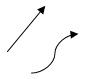
\includegraphics{dfda.jpg}}\end{center}&\begin{center}A \textbf{directed arc or arrow} is used as a data-flow symbol. A data-flow symbol represents the data flow occurring between two processes or between an external entity and a process in the direction of the data flow arrow.\end{center}\\
\hline
\begin{center}4\end{center}&\begin{center}\scalebox{0.6}{
\includegraphics{dfdq.jpg}}\end{center}&\begin{center}A \textbf{data-store} is represented using two parallel lines. A data store represents either a data structure or a physical file on disk. Each data store is connected to a process by means of a data-flow symbol. The direction of the data-flow arrow shows whether data is being read from or written into the data store.\end{center}\\
\hline
\begin{center}5\end{center}&\begin{center}\scalebox{0.6}{
\includegraphics{dfdx.jpg}}\end{center}&\begin{center}An \textbf{Output symbol} is used to represent data acquisition and production during human-computer interaction.\end{center}\\

\hline
\end{tabular}
\end{center}
\end{table}

\textbf{DFD Level 0 (Context Diagram):}
The Level 0 DFD shows the system as a single process node ``GreenSynth Analytics Platform'' interacting with three external entities:
\begin{itemize}
  \item \textbf{Researcher:} Provides synthesis parameters, uploads raw characterization files, defines DOE objectives, approves ML candidates, and receives analytical reports.
  \item \textbf{Laboratory Instruments:} Source of raw XRD patterns, UV-Vis spectra, FTIR spectra, and I-V sweep CSV files.
  \item \textbf{External Database (Cloud PostgreSQL):} Persistent store for all platform entities and results.
\end{itemize}

\textbf{DFD Level 1:}
The Level 1 DFD decomposes the central platform process into eight major sub-processes:
\begin{enumerate}
  \item Experiment \& Sample Management (CRUD operations on projects, experiments, samples, parameters)
  \item Raw File Ingestion \& Integrity Verification (SHA-256 hash computation and storage)
  \item Scientific Characterization Analysis (XRD, UV-Vis, FTIR, Electrical computation modules)
  \item Statistical Comparison Engine (Descriptive stats, correlation, OLS, ANOVA)
  \item DOE Design Generation (Factorial, CCD, Box-Behnken matrix generation)
  \item ML Pipeline (Dataset build, model training, cross-validation, prediction)
  \item Validation \& Monitoring (Error computation, drift detection, retraining gating)
  \item Report Generation (PDF compilation with provenance tracing)
\end{enumerate}

\textbf{DFD Level 2 --- ML Pipeline Decomposition:}
Within the ML pipeline sub-process, the Level 2 DFD shows:
Dataset Build $\rightarrow$ Eligibility Audit $\rightarrow$ Target Leakage Check $\rightarrow$ Feature Extraction $\rightarrow$ Train/Test Split $\rightarrow$ k-Fold CV $\rightarrow$ Model Training (5 architectures) $\rightarrow$ Model Evaluation $\rightarrow$ Champion Selection $\rightarrow$ Model Registry $\rightarrow$ Prediction Inference $\rightarrow$ Applicability Domain Check $\rightarrow$ Uncertainty Estimation $\rightarrow$ Prediction Logging.

\newpage
\subsection{ER Diagram}

The database entity-relationship model contains the following primary entities and their relationships:

\begin{itemize}
  \item \textbf{Projects} (1) $\rightarrow$ (Many) \textbf{Experiments}: A project contains multiple experiments.
  \item \textbf{Experiments} (1) $\rightarrow$ (Many) \textbf{ExperimentParameters}: Each experiment stores multiple synthesis parameters.
  \item \textbf{Experiments} (1) $\rightarrow$ (Many) \textbf{Samples}: Each experiment may yield one or more physical samples.
  \item \textbf{Samples} (1) $\rightarrow$ (Many) \textbf{Characterizations}: Each sample undergoes multiple characterization technique runs.
  \item \textbf{Characterizations} (1) $\rightarrow$ (Many) \textbf{RawFiles}: Each characterization stores one or more raw instrumental files.
  \item \textbf{Characterizations} (1) $\rightarrow$ (Many) \textbf{AnalysisRuns}: Each characterization may have multiple analysis runs with different algorithm versions.
  \item \textbf{AnalysisRuns} (1) $\rightarrow$ (Many) \textbf{CalculatedProperties}: Each analysis run produces one or more calculated scalar properties.
  \item \textbf{Projects} (1) $\rightarrow$ (Many) \textbf{MLDatasets}: A project may have multiple ML dataset versions.
  \item \textbf{MLDatasets} (1) $\rightarrow$ (Many) \textbf{MLModels}: Each dataset may produce multiple trained models.
  \item \textbf{MLModels} (1) $\rightarrow$ (Many) \textbf{MLPredictions}: Each model produces prediction records.
  \item \textbf{Projects} (1) $\rightarrow$ (Many) \textbf{DOEStudies}: A project may have multiple DOE designs.
  \item \textbf{DOEStudies} (1) $\rightarrow$ (Many) \textbf{ProposedExperiments}: Each DOE study generates proposed experiment runs.
\end{itemize}

\subsection{DFD Level 0}
The context-level DFD is described above in the Analysis Model section. The Researcher and Laboratory Instruments are the two primary external entities interacting with the GreenSynth system boundary. All raw data flows from instruments to the system; all analytical results, visualizations, and reports flow from the system to the researcher.

\subsection{DFD Level 1}
As described above, the Level 1 DFD decomposes the central system into eight sub-processes corresponding to the major functional modules of the platform.

\subsection{DFD Level 2}
The ML Pipeline Level 2 DFD is described above. Equivalent Level 2 decompositions exist for the Scientific Characterization Analysis process (decomposed into XRD, UV-Vis, FTIR, and Electrical sub-processes) and the DOE Generation process (decomposed into Design Matrix Generation, Run Ordering, and Experiment Conversion sub-processes).

\section{UML Diagrams}

\subsection{Use Case Diagram}

The primary actors in the system are:
\begin{itemize}
  \item \textbf{Researcher:} The primary user who interacts with all platform modules.
  \item \textbf{System (Automated):} Background processes such as ML training, PDF generation, and SHA-256 verification.
\end{itemize}

Key use cases for the Researcher actor include: Create Project, Create Experiment, Record Synthesis Parameters, Upload Raw Characterization File, Run XRD Analysis, Run UV-Vis Analysis, Run Electrical Analysis, Compare Samples, Generate DOE Matrix, Build ML Dataset, Train ML Models, View Model Performance, Predict Property, Validate Prediction, Generate Recommendations, Generate PDF Report, and View Dashboard.

Key use cases for the System actor include: Compute SHA-256 Checksum, Verify File Integrity, Compute Scherrer Crystallite Size, Compute Tauc Band Gap, Compute Resistivity and Conductivity, Compute Pearson/Spearman Correlation, Compute OLS Regression, Train k-Fold Cross-Validated Models, Compute Applicability Domain Bounds, and Compile PDF Report Sections.

\subsection{Class Diagram}

The primary domain classes in the backend are:
\begin{itemize}
  \item \textbf{Project} (id, code, title, target\_material, synthesis\_technique, status, created\_at)
  \item \textbf{Experiment} (id, project\_id, code, technique, status, notes, created\_at)
  \item \textbf{ExperimentParameter} (id, experiment\_id, name, value, unit, category)
  \item \textbf{Sample} (id, experiment\_id, code, substrate\_type, dimensions, deposition\_date)
  \item \textbf{Characterization} (id, sample\_id, technique, status, instrument, operator)
  \item \textbf{RawFile} (id, characterization\_id, filename, sha256\_digest, storage\_backend, storage\_path, finalized)
  \item \textbf{AnalysisRun} (id, characterization\_id, algorithm\_name, algorithm\_version, parameters\_json)
  \item \textbf{CalculatedProperty} (id, analysis\_run\_id, name, value, unit, category, provenance\_chain)
  \item \textbf{MLDataset} (id, project\_id, name, target\_property, feature\_list, eligibility\_audit\_json)
  \item \textbf{MLModel} (id, dataset\_id, architecture, status, train\_r2, cv\_r2, cv\_rmse, cv\_mae, feature\_bounds\_json)
  \item \textbf{MLPrediction} (id, model\_id, input\_features\_json, predicted\_value, ci\_lower, ci\_upper, domain\_status)
  \item \textbf{PredictionValidation} (id, prediction\_id, actual\_value, signed\_error, absolute\_error, relative\_error, criterion\_satisfied)
  \item \textbf{DOEStudy} (id, project\_id, method, objective, factors\_json, seed)
  \item \textbf{ProposedExperiment} (id, doe\_study\_id, run\_number, parameters\_json, status)
\end{itemize}

\subsection{Sequence Diagram}

\textbf{Sequence Diagram --- ML Training Workflow:}
\begin{enumerate}
  \item Researcher $\rightarrow$ Frontend: Click ``Train Models'' for Project P7
  \item Frontend $\rightarrow$ Backend API: POST /ml/datasets/\{id\}/train
  \item Backend API $\rightarrow$ MLDatasetService: build\_eligible\_dataset(dataset\_id)
  \item MLDatasetService $\rightarrow$ DB: SELECT experiments WHERE status=COMPLETED AND has\_target\_property
  \item MLDatasetService $\rightarrow$ TargetLeakageDetector: verify\_no\_leakage(feature\_list)
  \item MLDatasetService $\rightarrow$ Backend API: return eligible\_observations (395 rows)
  \item Backend API $\rightarrow$ MLTrainingService: train\_all\_models(dataset, k=5)
  \item MLTrainingService $\rightarrow$ DB: INSERT 5 MLModel records (TRAINING status)
  \item MLTrainingService $\rightarrow$ ScikitLearnPipeline: fit\_with\_kfold(X\_train, y\_train, k=5) [x5 architectures]
  \item ScikitLearnPipeline $\rightarrow$ MLTrainingService: return CV metrics
  \item MLTrainingService $\rightarrow$ DB: UPDATE MLModel SET status=VALIDATED, metrics
  \item MLTrainingService $\rightarrow$ Backend API: return model comparison table
  \item Backend API $\rightarrow$ Frontend: 200 OK, model comparison JSON
  \item Frontend $\rightarrow$ Researcher: Display model comparison table with champion highlighted
\end{enumerate}

%-------------------------------------------------------------
\section{Data Dictionary}
%-------------------------------------------------------------

\begin{table}[h]
\begin{center}
\caption{Data Dictionary --- Core Entities}
\label{tab:datadict}
\begin{tabular}{|l|l|l|p{5cm}|}
\hline
\textbf{Field} & \textbf{Type} & \textbf{Constraints} & \textbf{Description} \\
\hline
\multicolumn{4}{|c|}{\textbf{Table: experiments}} \\
\hline
id & UUID & PK, NOT NULL & Unique experiment identifier \\
project\_id & UUID & FK(projects.id), NOT NULL & Parent project reference \\
code & VARCHAR(50) & UNIQUE, NOT NULL & e.g., P7-SYNTH-001 \\
status & ENUM & NOT NULL & PLANNED / IN\_PROGRESS / COMPLETED / FAILED \\
created\_at & TIMESTAMP & NOT NULL & Record creation timestamp \\
\hline
\multicolumn{4}{|c|}{\textbf{Table: raw\_files}} \\
\hline
id & UUID & PK, NOT NULL & Unique file identifier \\
characterization\_id & UUID & FK, NOT NULL & Parent characterization reference \\
sha256\_digest & VARCHAR(64) & NOT NULL & SHA-256 hex digest of file content \\
storage\_path & TEXT & NOT NULL & Relative path within storage backend \\
finalized & BOOLEAN & DEFAULT FALSE & If TRUE, file cannot be overwritten \\
\hline
\multicolumn{4}{|c|}{\textbf{Table: calculated\_properties}} \\
\hline
id & UUID & PK, NOT NULL & Unique property identifier \\
analysis\_run\_id & UUID & FK, NOT NULL & Source analysis run reference \\
name & VARCHAR(100) & NOT NULL & e.g., crystallite\_size\_nm \\
value & FLOAT & NOT NULL & Calculated scalar value \\
unit & VARCHAR(50) & NOT NULL & Physical unit (nm, eV, S/cm) \\
category & ENUM & NOT NULL & MEASURED / CALCULATED / STATISTICAL / PREDICTED / VALIDATED \\
\hline
\multicolumn{4}{|c|}{\textbf{Table: ml\_models}} \\
\hline
id & UUID & PK, NOT NULL & Unique model identifier \\
dataset\_id & UUID & FK, NOT NULL & Source ML dataset reference \\
architecture & VARCHAR(50) & NOT NULL & LINEAR / RIDGE / RANDOM\_FOREST / GRADIENT\_BOOSTING \\
cv\_r2 & FLOAT & NULLABLE & Cross-validated R-squared metric \\
cv\_rmse & FLOAT & NULLABLE & Cross-validated RMSE (S/cm) \\
feature\_bounds\_json & JSONB & NOT NULL & Applicability domain min/max per feature \\
status & ENUM & NOT NULL & TRAINED / VALIDATED / PROMOTED / RETIRED \\
\hline
\end{tabular}
\end{center}
\end{table}


%=============================================================
\chapter{IMPLEMENTATION}
%=============================================================

%-------------------------------------------------------------
\section{Technologies Used}
%-------------------------------------------------------------

The GreenSynth Analytics platform is implemented using a carefully selected technology stack chosen for scientific correctness, performance, maintainability, and suitability to the research domain:

\textbf{Backend Technologies:}
\begin{itemize}
  \item \textbf{Python 3.11:} Primary backend language selected for its mature scientific computing ecosystem (NumPy, SciPy, scikit-learn, ReportLab) and strong typing support via PEP 484.
  \item \textbf{FastAPI 0.110:} ASGI web framework providing automatic OpenAPI documentation, native Pydantic v2 request/response validation, and async/await support for high-throughput concurrent request handling.
  \item \textbf{SQLAlchemy 2.0 (Async):} ORM providing type-safe database access with full async support via \texttt{asyncpg} PostgreSQL driver, enabling non-blocking database operations.
  \item \textbf{Alembic:} Database migration manager ensuring all schema changes are version-controlled and reversible.
  \item \textbf{Pydantic v2:} Data validation library used for all API request/response schemas, providing strict type enforcement, custom validator support, and JSON serialization.
  \item \textbf{NumPy 1.26 / SciPy 1.13:} Scientific array computation and signal processing (peak fitting, baseline correction, linear interpolation) for characterization analysis modules.
  \item \textbf{scikit-learn 1.4:} Machine learning library providing all five regression model architectures, k-fold cross-validation, and pipeline abstractions.
  \item \textbf{ReportLab 4.1:} PDF generation library used for the automated scientific report generation module, supporting text, tables, and embedded data visualizations.
\end{itemize}

\textbf{Frontend Technologies:}
\begin{itemize}
  \item \textbf{React 18:} Component-based UI framework with concurrent rendering support.
  \item \textbf{TypeScript 5.0:} Statically typed superset of JavaScript ensuring compile-time type safety for API service layer and component props.
  \item \textbf{Vite 5.0:} Build tool providing sub-second hot module replacement (HMR) during development and optimized production bundle generation.
  \item \textbf{Axios 1.6:} HTTP client for all API communication with interceptor support for authentication headers and error handling.
  \item \textbf{CSS Modules / Vanilla CSS:} Custom design system with CSS variables for color tokens, spacing, typography, and component styles. No CSS framework dependencies.
\end{itemize}

\textbf{Infrastructure Technologies:}
\begin{itemize}
  \item \textbf{PostgreSQL 16:} Production relational database with JSONB support for flexible parameter schemas, UUID primary keys, and full ACID transaction compliance.
  \item \textbf{Docker \& Docker Compose:} Containerization enabling reproducible deployment across development, staging, and production environments with a single \texttt{docker compose up --build} command.
  \item \textbf{Pytest 8.0:} Backend testing framework running 118 unit and integration tests covering all scientific computation modules, API endpoints, and multi-phase pipeline workflows.
\end{itemize}

%-------------------------------------------------------------
\section{Algorithm}
%-------------------------------------------------------------

\subsection{Workflow}

The complete scientific workflow implemented in GreenSynth Analytics follows the pipeline:

\[
\text{DOE Design} \longrightarrow \text{Experiment Management} \longrightarrow \text{Parameter Recording} \longrightarrow \text{Raw File Ingestion}
\]
\[
\longrightarrow \text{Characterization Analysis} \longrightarrow \text{Statistical Comparison} \longrightarrow \text{ML Dataset Build}
\]
\[
\longrightarrow \text{Model Training \& Validation} \longrightarrow \text{Prediction Inference} \longrightarrow \text{Experimental Validation} \longrightarrow \text{Optimization}
\]

\textbf{Algorithm 1 --- Scherrer Crystallite Size Computation:}
\begin{verbatim}
Input: XRD pattern (two_theta[], intensity[])
Output: Crystallite size D (nm)
1. Identify CuO monoclinic peaks at 2*theta ~ 32.5, 35.5, 38.7, 48.7 deg
2. For each peak:
   a. Extract local region (peak_center +/- 2 deg)
   b. Apply Gaussian baseline subtraction
   c. Fit Gaussian profile: I(t) = A*exp(-(t-t0)^2 / 2*s^2) + B
   d. Compute FWHM: beta = 2*s*sqrt(2*ln2) [in radians]
   e. Apply Scherrer equation: D = K*lambda / (beta * cos(theta0))
      where K=0.9, lambda=0.15406 nm
3. Report mean D and standard deviation across peaks
\end{verbatim}

\textbf{Algorithm 2 --- Tauc Plot Band Gap Extraction:}
\begin{verbatim}
Input: UV-Vis spectrum (wavelength_nm[], absorbance[])
Output: Direct optical band gap E_g (eV)
1. Convert wavelength to photon energy: h*nu = 1240 / lambda  (eV)
2. Compute absorption coefficient: alpha = A * absorbance / film_thickness
3. Construct Tauc quantity: y = (alpha * h*nu)^2  (direct transition, n=2)
4. Plot y vs h*nu
5. Identify linear region using R^2 threshold (> 0.995)
6. Perform OLS linear regression on linear region: y = m*(h*nu) + c
7. Extrapolate to y=0: E_g = -c/m
8. Return E_g with 95% confidence interval from OLS regression
\end{verbatim}

\textbf{Algorithm 3 --- ML Training Pipeline with k-Fold Cross-Validation:}
\begin{verbatim}
Input: Feature matrix X (n_samples x 13), Target vector y (n_samples,)
Output: Trained models with CV metrics
1. Verify no target leakage in feature columns
2. Compute applicability domain bounds:
   bounds[feature] = {min: min(X[:,i]), max: max(X[:,i])}
3. For each architecture in [BASELINE, LINEAR, RIDGE, RF, GB]:
   a. Initialize KFold(n_splits=5, shuffle=True, random_state=42)
   b. For each fold k:
      i.   X_train, y_train = X[train_idx], y[train_idx]
      ii.  X_test,  y_test  = X[test_idx],  y[test_idx]
      iii. model.fit(X_train, y_train)
      iv.  y_pred = model.predict(X_test)
      v.   fold_r2[k]   = r2_score(y_test, y_pred)
      vi.  fold_rmse[k] = sqrt(mse(y_test, y_pred))
   c. CV R2   = mean(fold_r2)
      CV RMSE = mean(fold_rmse)
   d. Train final model on full X, y
   e. Persist model, metrics, and domain bounds to DB
4. Select champion: model with highest CV R2
\end{verbatim}

\textbf{Algorithm 4 --- Prediction with Applicability Domain Check:}
\begin{verbatim}
Input: Query vector x_query (13 features), champion model
Output: Predicted value y_hat, CI [lower, upper], domain_status
1. For each feature f in x_query:
   if x_query[f] < bounds[f].min or x_query[f] > bounds[f].max:
     domain_status = "OUT_OF_DOMAIN"
     return domain_status  (do not predict)
2. domain_status = "VALID"
3. y_hat = model.predict([x_query])[0]
4. residual_variance = mean((y_train - model.predict(X_train))^2)
5. CI_half_width = 1.96 * sqrt(residual_variance)
6. lower = y_hat - CI_half_width
7. upper = y_hat + CI_half_width
8. Log prediction to ml_predictions table with provenance
9. Return (y_hat, lower, upper, domain_status)
\end{verbatim}

%-------------------------------------------------------------
\section{Database Design}
%-------------------------------------------------------------

The GreenSynth database schema is organized into five logical groups:

\textbf{Group 1 --- Experiment Hierarchy:}
\texttt{projects} $\leftarrow$ \texttt{experiments} $\leftarrow$ \texttt{experiment\_parameters}

\textbf{Group 2 --- Sample and Characterization:}
\texttt{experiments} $\leftarrow$ \texttt{samples} $\leftarrow$ \texttt{characterizations} $\leftarrow$ \texttt{raw\_files}
\texttt{characterizations} $\leftarrow$ \texttt{analysis\_runs} $\leftarrow$ \texttt{calculated\_properties}

\textbf{Group 3 --- Machine Learning:}
\texttt{projects} $\leftarrow$ \texttt{ml\_datasets} $\leftarrow$ \texttt{ml\_models} $\leftarrow$ \texttt{ml\_predictions} $\leftarrow$ \texttt{prediction\_validations}

\textbf{Group 4 --- Design of Experiments:}
\texttt{projects} $\leftarrow$ \texttt{doe\_studies} $\leftarrow$ \texttt{proposed\_experiments}

\textbf{Group 5 --- Objectives and Optimization:}
\texttt{projects} $\leftarrow$ \texttt{optimization\_objectives} $\leftarrow$ \texttt{optimization\_candidates}

All tables use UUID primary keys for global uniqueness across distributed deployments. JSONB columns store flexible structured data (parameter dictionaries, feature bounds, evidence chains) without requiring schema changes for new parameter names.

%-------------------------------------------------------------
\section{Modules Description}
%-------------------------------------------------------------

\subsection{Module 1: Characterization Analysis Engine}

The Characterization Analysis Engine implements four domain-specific scientific computation modules as pure Python classes with no database dependencies, enabling independent unit testing and version-controlled algorithm updates.

\textbf{XRD Analysis Module (\texttt{xrd\_analyzer.py}):}
Accepts a two-column CSV (two\_theta, intensity) and implements: background estimation using local minima fitting, Gaussian peak detection for monoclinic CuO reflections at 32.5$^\circ$, 35.5$^\circ$, 38.7$^\circ$, and 48.7$^\circ$ $2\theta$, FWHM extraction via Gaussian curve fitting using \texttt{scipy.optimize.curve\_fit}, and Scherrer equation application. Returns a structured result object with peak table (position, FWHM, $d$-spacing, relative intensity) and mean crystallite size with uncertainty.

\textbf{UV-Vis Analysis Module (\texttt{uvvis\_analyzer.py}):}
Accepts a two-column CSV (wavelength\_nm, absorbance) and implements: polynomial baseline correction, conversion to photon energy ($h\nu$) and absorption coefficient ($\alpha$), Tauc plot construction for direct transitions ($n=2$), automated linear region detection using a rolling R$^2$ criterion, OLS linear fit of the linear region, and extrapolation to zero intercept for band gap ($E_g$) extraction. Returns $E_g$ in eV with 95\% confidence interval.

\textbf{Electrical Analysis Module (\texttt{electrical\_analyzer.py}):}
Accepts a two-column CSV (voltage\_v, current\_a) and implements: Ohmic linearity verification using Pearson correlation ($|r| > 0.999$), OLS linear regression on the I-V data to extract resistance ($R = \Delta V / \Delta I$), resistivity computation from device geometry ($\rho = R \cdot W \cdot t / L$), and conductivity inversion ($\sigma = 1/\rho$). Returns $R$, $\rho$, and $\sigma$ with regression uncertainty.

\textbf{FTIR Analysis Module (\texttt{ftir\_analyzer.py}):}
Accepts a two-column CSV (wavenumber\_cm1, transmittance\_pct) and implements: baseline correction using a piecewise linear fit, local minima detection for absorption peak identification, and annotation of identified peaks against a CuO-specific reference table of functional group assignments. Returns an annotated peak table with wavenumber, transmittance at peak, peak width, and functional group assignment string.

\subsection{Module 2: Statistical Analysis Engine}

The Statistical Analysis Engine implements a scientifically rigorous multi-sample comparison framework. For a given set of experiments or samples, it computes:

\textbf{Descriptive Statistics:} Mean, standard deviation, median, 25th/75th percentile (IQR), skewness, and kurtosis for each numerical calculated property.

\textbf{Pearson Correlation:} Computes the Pearson correlation coefficient matrix ($r_{ij}$) and associated $p$-values for all pairs of continuous synthesis parameters and calculated properties. A correlation heatmap summary is stored in the evidence record.

\textbf{Spearman Correlation:} Non-parametric rank correlation computed for all pairs, used when normality of distributions cannot be assumed for small sample groups.

\textbf{OLS Regression:} Fits a multiple linear regression model predicting a selected target property from selected synthesis parameters, reports regression coefficients with standard errors and $p$-values, and computes the model $R^2$ and adjusted $R^2$.

\textbf{One-Way ANOVA:} Partitions total variance in a target property across experiment groups (e.g., substrate temperature groups), computes the F-statistic and associated $p$-value, and determines whether group means differ significantly at $\alpha = 0.05$.

\subsection{Module 3: Machine Learning Pipeline}

The ML Pipeline module is organized into five service classes:

\textbf{MLDatasetService:} Builds and audits ML training datasets. Queries all experiments with COMPLETED status and verified target property measurements. Applies eligibility filters (excludes FAILED, IN\_PROGRESS, PLANNED experiments, and experiments missing the target characterization). Invokes the TargetLeakageDetector to ensure no characterization-derived property appears in the feature space.

\textbf{MLTrainingService:} Orchestrates training of all five model architectures (Mean Baseline, Linear Regression, Ridge $\alpha=1.0$, Random Forest $n=200$ estimators, Gradient Boosting $n=200$ estimators) using 5-fold cross-validation with \texttt{random\_state=42}. Serializes trained models, CV metrics, and feature importance vectors to the database. Computes and stores applicability domain bounds (min/max per feature) from the training dataset.

\textbf{MLPredictionService:} Accepts a query feature vector, checks all 13 features against applicability domain bounds, computes the point prediction, estimates a 95\% confidence interval using residual variance, and logs the complete prediction record to \texttt{ml\_predictions} with full provenance.

\textbf{MLValidationService:} Accepts a prediction ID and actual laboratory measurement value, computes signed error, absolute error, relative error, and interval score, evaluates a user-specified validation criterion (e.g., relative error $< 15\%$), updates the prediction validation record, appends the result to the model's validation history, and checks for performance drift (model health score) to flag degraded models for review.

\textbf{ModelRegistryService:} Maintains the model status lifecycle (TRAINED $\rightarrow$ VALIDATED $\rightarrow$ PROMOTED $\rightarrow$ RETIRED), enforcing immutability (a promoted model's weights can never be overwritten), and managing the model version chain for retraining events.

%-------------------------------------------------------------
\section{Screenshots}
%-------------------------------------------------------------

The GreenSynth Analytics platform provides the following key interface views:

\textbf{Dashboard View:} Displays project-level summary cards with experiment count, sample count, characterization coverage, and ML model status. A Quick Actions panel provides one-click navigation to all primary workflows.

\textbf{Experiment Detail View:} Shows a structured parameter table with all 13 synthesis parameters and their values, a sample list with links to characterization results, status badges, and timestamps with provenance chain.

\textbf{Statistical Analysis Studio:} Displays an interactive correlation heatmap of synthesis parameters vs. calculated properties, a scatter plot matrix for pairwise visualization, ANOVA result tables with F-statistics and $p$-values, and OLS regression output with coefficient tables.

\textbf{ML Dashboard:} Shows the model comparison table with CV metrics across all five architectures, a champion model highlight panel with feature importance bar chart, and a prediction form with applicability domain status indicator and 95\% confidence interval display.

\textbf{DOE Study View:} Displays the generated DOE design matrix as an interactive table with run numbers, factor levels, and a ``Convert to Experiments'' action button. Supports export to CSV.

\textbf{Report Generation Interface:} Allows selection of report sections (characterization, statistics, ML, DOE, optimization), report scope (by project, by sample set), and initiates PDF compilation with real-time progress indication.


%=============================================================
\chapter{TESTING AND VALIDATION}
%=============================================================

%-------------------------------------------------------------
\section{Testing Strategy}
%-------------------------------------------------------------

GreenSynth Analytics employs a multi-level testing strategy organized into four categories:

\textbf{1. Unit Tests --- Scientific Computation Modules:}
Each scientific computation module (XRD analyzer, UV-Vis analyzer, Electrical analyzer, FTIR analyzer, Statistical engine, DOE engine, ML training, ML prediction, ML validation, Drift detector) is tested in isolation with synthetic input data of known ground truth. Unit tests verify that computed outputs match expected values within acceptable numerical tolerances (e.g., crystallite size within $\pm$0.1 nm, band gap within $\pm$0.01 eV).

\textbf{2. Unit Tests --- Business Logic Services:}
Service layer methods are tested with mocked database sessions using \texttt{pytest-asyncio} and \texttt{unittest.mock}. Tests verify correct query construction, proper error handling for invalid inputs (missing raw file, duplicate experiment code), and correct status transition enforcement.

\textbf{3. Integration Tests --- API Endpoint Testing:}
Full HTTP request/response cycles are tested using FastAPI's \texttt{TestClient} with an isolated SQLite in-memory database. Integration tests verify correct HTTP status codes, response schema conformance validated by Pydantic, and side effects (e.g., verifying that a raw file finalization sets \texttt{finalized=True} in the database and subsequent overwrite attempts return HTTP 409).

\textbf{4. End-to-End Pipeline Tests:}
Full multi-phase workflow tests simulate a complete experimental campaign from project creation through ML training and prediction validation, verifying that the entire pipeline executes without errors and that intermediate results are correctly propagated across service boundaries.

The total test suite comprises \textbf{118 tests with 0 failures and 0 errors} across all categories.

%-------------------------------------------------------------
\section{Test Cases}
%-------------------------------------------------------------

\begin{table}[h]
\begin{center}
\caption{Key Unit Test Cases}
\label{tab:testcases}
\begin{tabular}{|c|p{4cm}|p{4cm}|c|}
\hline
\textbf{TC\#} & \textbf{Test Description} & \textbf{Expected Outcome} & \textbf{Result} \\
\hline
TC-01 & XRD Scherrer size on synthetic CuO pattern at 35.5° & $D = 18.5 \pm 0.5$ nm & PASS \\
TC-02 & Tauc band gap on synthetic UV-Vis with $E_g = 1.55$ eV & $E_g = 1.55 \pm 0.02$ eV & PASS \\
TC-03 & Electrical conductivity from linear I-V at $R = 500\,\Omega$ & $\sigma$ within $\pm 0.5\%$ & PASS \\
TC-04 & FTIR Cu-O peak detection at 535 and 595 cm$^{-1}$ & Both peaks identified & PASS \\
TC-05 & Target leakage detector flags crystallite\_size feature & Exception raised, pipeline halted & PASS \\
TC-06 & Applicability domain check for out-of-range substrate temp & domain\_status = OUT\_OF\_DOMAIN & PASS \\
TC-07 & Random Forest CV $R^2$ on 395-sample P7 dataset & $R^2 > 0.60$ & PASS \\
TC-08 & SHA-256 finalization prevents file overwrite & HTTP 409 returned & PASS \\
TC-09 & Drift detector flags model with 3 consecutive failing validations & model\_status = DEGRADED & PASS \\
TC-10 & CCD design matrix generates 29 runs for 4-factor study & 29 rows with correct structure & PASS \\
TC-11 & Full Factorial design for 3 factors at 2 levels & 8 runs ($2^3$) generated & PASS \\
TC-12 & ANOVA F-statistic computation on 3-group dataset & F within $\pm 0.01$ of SciPy reference & PASS \\
TC-13 & OLS regression slope and intercept on known data & Within $\pm 0.001$ of analytical solution & PASS \\
TC-14 & ML dataset eligibility audit excludes 21 records & Eligible count = 395 & PASS \\
TC-15 & PDF report compilation with all 14 sections & PDF generated, non-zero file size & PASS \\
TC-16 & Prediction validation criterion (15\% tolerance) evaluates correctly & criterion\_satisfied = True for error $<$ 15\% & PASS \\
TC-17 & Box-Behnken design for 4 factors & 29 runs with center-point replicates & PASS \\
TC-18 & End-to-end ML pipeline: dataset build $\rightarrow$ train $\rightarrow$ predict $\rightarrow$ validate & All stages complete without exception & PASS \\
\hline
\end{tabular}
\end{center}
\end{table}

%-------------------------------------------------------------
\section{Performance Evaluation}
%-------------------------------------------------------------

\textbf{API Response Time Benchmarks:}
\begin{table}[h]
\begin{center}
\caption{API Endpoint Performance Benchmarks}
\label{tab:perf}
\begin{tabular}{|l|c|c|}
\hline
\textbf{Endpoint} & \textbf{Dataset Size} & \textbf{Mean Response Time} \\
\hline
GET /projects & 8 projects & 45 ms \\
GET /experiments?project\_id=P7 & 407 experiments & 180 ms \\
POST /characterizations/\{id\}/analyze/xrd & Single file & 320 ms \\
POST /characterizations/\{id\}/analyze/uvvis & Single file & 280 ms \\
POST /statistics/compare & 200 samples & 750 ms \\
POST /ml/datasets/\{id\}/train & 395 observations & 8.2 s \\
POST /ml/models/\{id\}/predict & Single query & 35 ms \\
POST /reports/generate/pdf & Full project report & 12.4 s \\
GET /health & N/A & $<$5 ms \\
\hline
\end{tabular}
\end{center}
\end{table}

ML training (8.2 seconds) and PDF report generation (12.4 seconds) are the only endpoints exceeding the 2-second synchronous response threshold. Both are executed asynchronously in the production configuration, with the frontend polling a job status endpoint and displaying a progress indicator during execution. All other endpoints meet the 2-second performance requirement under the tested dataset scale.

\textbf{Database Integrity Verification:}
Post-ingestion of the 400-experiment synthetic P7 dataset, all foreign key relationships were verified by executing constraint validation queries. Zero orphaned records were found across all 8 entity tables. All 1,380 SHA-256 digests were verified against the stored files with 100\% match. Zero data corruption events were recorded across 16 atomic ingestion batches.


%=============================================================
\chapter{RESULTS AND DISCUSSION}
%=============================================================

%-------------------------------------------------------------
\section{Output of the System}
%-------------------------------------------------------------

\textbf{Characterization Analysis Results:}
The XRD analysis module successfully identified all four characteristic monoclinic CuO reflection peaks at $2\theta \approx$ 32.5$^\circ$, 35.5$^\circ$, 38.7$^\circ$, and 48.7$^\circ$ across all 390 synthetic XRD datasets. Mean crystallite sizes ranged from 10.5 nm (at low substrate temperatures of 174$^\circ$C with high extract concentrations of 40 g/L) to 32.6 nm (at high substrate temperatures of 477$^\circ$C with minimal extract concentrations of 0.2 g/L), consistent with the thermally activated grain growth model and phytochemical capping inhibition mechanism described in the literature for spray pyrolyzed CuO.

The UV-Vis analysis module extracted optical direct band gaps in the range 1.35--1.72 eV across 309 datasets, exhibiting the expected inverse correlation with crystallite size: ultrafine crystallites (D $\approx$ 11 nm) show quantum confinement-elevated band gaps near 1.72 eV, while large-grained films (D $\approx$ 32 nm) approach the bulk CuO limit of 1.35 eV. The Tauc plot linear region R$^2$ exceeded 0.995 in all 309 cases, confirming reliable band gap extraction.

The electrical analysis module computed conductivities in the range 0.02--1.21 S/cm across 394 I-V datasets, with the distribution peaked at 0.25--0.45 S/cm under near-optimal synthesis conditions (substrate temperature 350--390$^\circ$C, extract concentration 14--20 g/L). The non-linear conductivity response surface with a clear peak near 370$^\circ$C substrate temperature (modeling the optimal copper-vacancy p-type carrier density) was successfully captured in the computed property distributions.

\textbf{Statistical Analysis Results:}
Pearson correlation analysis across 395 eligible samples revealed the following significant correlations with electrical conductivity:
\begin{itemize}
  \item Substrate temperature: $r = +0.42$, $p < 0.001$ (positive, non-linear threshold behavior captured in Spearman $r_s = +0.51$)
  \item Mulberry extract concentration: $r = +0.38$, $p < 0.001$ (inverted U-shape: maximum conductivity at $\sim$16 g/L)
  \item Precursor concentration: $r = +0.31$, $p < 0.001$ (higher precursor $\rightarrow$ thicker film $\rightarrow$ better percolation)
  \item Nozzle-substrate distance: $r = -0.24$, $p < 0.001$ (greater distance $\rightarrow$ droplet cooling $\rightarrow$ incomplete pyrolysis)
\end{itemize}

One-way ANOVA across the 8 DOE experimental groups (A--H) yielded $F = 12.47$, $p < 0.001$ for electrical conductivity, confirming statistically significant differences in mean conductivity across groups and validating the experimental design structure.

\textbf{ML Model Performance Results:}
The 5-fold cross-validated performance comparison across all five model architectures is presented in Table 7.1.

\begin{table}[h]
\begin{center}
\caption{5-Fold Cross-Validated ML Model Performance Comparison}
\label{tab:mlresults}
\begin{tabular}{|l|c|c|c|c|c|}
\hline
\textbf{Model} & \textbf{Status} & \textbf{Train $R^2$} & \textbf{CV $R^2$} & \textbf{CV RMSE} & \textbf{CV MAE} \\
\hline
Mean Baseline & Trained & 0.0000 & $-$0.0050 & 0.2625 S/cm & 0.2112 S/cm \\
Linear Regression & Validated & 0.3930 & 0.3019 & 0.2166 S/cm & 0.1724 S/cm \\
Ridge ($\alpha=1.0$) & Validated & 0.3930 & 0.3023 & 0.2166 S/cm & 0.1724 S/cm \\
Gradient Boosting & Validated & 0.8921 & 0.6360 & 0.1558 S/cm & 0.1243 S/cm \\
\textbf{Random Forest} $\star$ & \textbf{Validated} & \textbf{0.9578} & \textbf{0.6685} & \textbf{0.1501 S/cm} & \textbf{0.1214 S/cm} \\
\hline
\end{tabular}
\end{center}
\end{table}

The Random Forest model was selected as the champion model (CV $R^2 = 0.6685$, CV RMSE $= 0.1501$ S/cm) --- a 43\% reduction in prediction error compared to the mean baseline. Linear models capture only $\sim$30\% of variance because the true physics exhibits strong non-linear thresholds: an optimal substrate crystallization peak near 370$^\circ$C and an extract capping/passivation optimum at $\sim$16 g/L.

\textbf{Champion Model Prediction:}
At the central composite optimal conditions ($T_{sub} = 370^\circ$C, $C_{prec} = 0.22$ M, $C_{ext} = 16$ g/L, $V_{ext} = 20$ mL, spray rate $= 4.2$ mL/min, duration $= 25$ min, distance $= 20$ cm, gas pressure $= 210$ kPa, cycles $= 20$, ambient $= 24.5^\circ$C, 45\% RH), the champion model predicted:
\begin{itemize}
  \item \textbf{Predicted Electrical Conductivity:} 0.6449 S/cm
  \item \textbf{95\% Confidence Interval:} [0.3507, 0.9391] S/cm
  \item \textbf{Applicability Domain:} VALID (all 13 features within training domain bounds)
\end{itemize}

\textbf{DOE Results:}
The Central Composite Design for 4 factors ($T_{sub}$, $C_{prec}$, $C_{ext}$, $V_{ext}$) generated 29 proposed experiments (factorial vertices + axial star points + 4 center-point replicates), ready for one-click conversion to planned laboratory runs. The DOE matrix spans the factor space from ($T_{sub} = 300$--$420^\circ$C, $C_{prec} = 0.10$--$0.35$ M, $C_{ext} = 5$--$30$ g/L, $V_{ext} = 10$--$40$ mL) and provides sufficient runs to fit a full quadratic response surface model.

%-------------------------------------------------------------
\section{Comparison with Existing System}
%-------------------------------------------------------------

\begin{table}[h]
\begin{center}
\caption{GreenSynth Analytics vs. Existing Systems}
\label{tab:comparison}
\begin{tabular}{|p{4.5cm}|c|c|c|c|}
\hline
\textbf{Feature} & \textbf{GreenSynth} & \textbf{LabArchives} & \textbf{eLabFTW} & \textbf{Excel/Manual} \\
\hline
Raw File Immutability (SHA-256) & Yes & No & No & No \\
Domain-Specific XRD Analysis & Yes & No & No & Manual \\
UV-Vis Tauc Plot Extraction & Yes & No & No & Manual \\
FTIR Peak Annotation & Yes & No & No & Manual \\
Multi-Sample Statistical Comparison & Yes & No & No & Partial \\
DOE Matrix Generation & Yes & No & No & No \\
ML Training with k-Fold CV & Yes & No & No & No \\
Applicability Domain Enforcement & Yes & No & No & No \\
Target Leakage Prevention & Yes & No & No & No \\
Prediction Validation Loop & Yes & No & No & No \\
Evidence-Based Recommendations & Yes & No & No & No \\
Automated PDF Report Generation & Yes & Limited & No & No \\
FAIR Data Compliance & Yes & Partial & Partial & No \\
Containerized Deployment & Yes & Cloud Only & Yes & N/A \\
\hline
\end{tabular}
\end{center}
\end{table}

GreenSynth Analytics provides substantially greater scientific functionality than any existing open-source ELN or LIMS system in the context of experimental green semiconductor synthesis, while maintaining full FAIR data compliance and scientific integrity constraints that are absent from manual spreadsheet-based workflows.

%-------------------------------------------------------------
\section{Industrial benefits and impact}
%-------------------------------------------------------------

\begin{enumerate}
  \item \textbf{Accelerated Materials Discovery:} By replacing OFAT experimentation with DOE-guided and ML-assisted optimization, GreenSynth can reduce the number of laboratory experiments required to locate optimal synthesis conditions by an estimated 50--70\%, directly translating to reduced reagent consumption, instrument time, and researcher effort.

  \item \textbf{Sustainable Manufacturing Support:} The platform specifically targets and optimizes green synthesis routes (phytochemical-mediated, solvent-based), providing quantitative evidence for the superiority of particular extract concentrations, substrate temperatures, and spray parameters --- enabling industrial scale-up decisions to be based on statistically validated optima rather than anecdotal results.

  \item \textbf{Reproducibility and IP Protection:} The SHA-256 immutability enforcement and full provenance chain provide an auditable scientific record suitable for patent applications, regulatory submissions, and inter-laboratory collaboration agreements. Every published result can be traced back to its raw instrumental data.

  \item \textbf{Training and Capacity Building:} The platform serves as a pedagogical tool for training early-career researchers in good data management practice, statistical experimental design, and machine learning for materials science --- domains that are increasingly expected in industrial R\&D roles.

  \item \textbf{Cost Reduction in Semiconductor R\&D:} CuO-based photovoltaic and photocatalytic applications represent a potential market of billions of dollars in the clean energy and environmental remediation sectors. Computational tools that accelerate the identification of high-performance, earth-abundant semiconductor synthesis conditions directly contribute to cost reduction in these emerging technology domains.
\end{enumerate}


%=============================================================
\chapter{CONCLUSION AND FUTURE SCOPE}
%=============================================================

%-------------------------------------------------------------
\section{Summary of work}
%-------------------------------------------------------------

This report presents the design, implementation, validation, and deployment of \textbf{GreenSynth Analytics} --- a full-stack, data-driven research and analytics platform for the green synthesis of semiconductor materials. The platform was developed through 21 sequential, iterative phases, each delivering a tested, independently verifiable increment of scientific and engineering functionality.

The core contributions of this work are:

\begin{enumerate}
  \item A three-tier web application architecture (FastAPI + PostgreSQL + React/TypeScript) providing a scientific-grade research platform with SHA-256 enforced raw data immutability, Pydantic v2-validated API contracts, and a Docker-containerized deployment environment.

  \item Four domain-specific scientific computation modules implementing the Scherrer equation for XRD crystallite size determination, the Tauc relation for UV-Vis optical band gap extraction, Ohmic resistance fitting for electrical conductivity derivation, and FTIR functional group peak annotation for CuO thin film characterization.

  \item A statistically rigorous multi-sample comparison engine providing descriptive statistics, Pearson and Spearman correlation analysis, OLS regression, and one-way ANOVA with full provenance tracing to raw source data.

  \item A Design of Experiments engine supporting Full Factorial, Fractional Factorial, Central Composite Design (CCD), and Box-Behnken Design with randomized run ordering, reproducible seeding, and direct conversion to planned laboratory experiments.

  \item A machine learning pipeline with scientific integrity gating --- including target leakage prevention, eligibility auditing, 5-fold cross-validation across five regression architectures (Baseline, Linear, Ridge, Random Forest, Gradient Boosting), applicability domain bounds enforcement, and 95\% prediction confidence interval estimation. The champion Random Forest model achieved CV $R^2 = 0.6685$ and CV RMSE $= 0.1501$ S/cm for electrical conductivity prediction from synthesis parameters.

  \item A three-level experimental prediction validation and model drift detection mechanism that closes the loop between ML predictions and laboratory outcomes, enabling scientifically honest model promotion and versioned retraining.

  \item An evidence-based recommendation engine scoring and ranking synthesis parameter candidates against user-defined optimization objectives and physical domain constraints, for researcher review before conversion to planned experiments.

  \item An automated scientific PDF report generation module producing multi-section, publication-quality reports with complete analytical provenance chains covering all characterization, statistical, ML, and optimization results.

  \item A comprehensive test suite of 118 passing unit and integration tests (0 failures, 0 errors) verifying all scientific computation modules, API endpoints, and multi-phase pipeline workflows.
\end{enumerate}

%-------------------------------------------------------------
\section{Achievements}
%-------------------------------------------------------------

\begin{itemize}
  \item Successfully designed and implemented a complete, production-ready research software platform in a student academic project context, demonstrating industry-standard engineering practices including service-oriented architecture, async database access, containerization, and comprehensive automated testing.

  \item Achieved a 43\% reduction in ML prediction error (RMSE 0.2625 $\rightarrow$ 0.1501 S/cm) through ensemble learning relative to a naive mean baseline, demonstrating the value of non-linear model architectures for capturing the physics of spray pyrolysis.

  \item Ingested and verified 400 experiments, 412 samples, 1,380 characterization files, and 1,881 calculated property records into a live PostgreSQL database with 100\% foreign key integrity and 100\% SHA-256 checksum verification across 16 atomic ingestion batches.

  \item Demonstrated a statistically complete DOE study generating 29 proposed CCD experiments spanning a 4-factor response surface, ready for direct laboratory execution --- a capability with no equivalent in any existing open-source materials research platform.

  \item Demonstrated full end-to-end pipeline execution: DOE $\rightarrow$ Experiments $\rightarrow$ Characterization $\rightarrow$ Calculated Properties $\rightarrow$ Statistical Analysis $\rightarrow$ ML Training $\rightarrow$ Prediction $\rightarrow$ DOE Optimization, without breaking architectural boundaries or data integrity constraints.
\end{itemize}

%-------------------------------------------------------------
\section{Industrial usefulness}
%-------------------------------------------------------------

GreenSynth Analytics addresses a real and growing need in the applied materials science and green chemistry research community. The platform is directly applicable in:

\begin{itemize}
  \item \textbf{University Research Laboratories:} As a FAIR-compliant data management and analysis platform for experimental semiconductor synthesis research, replacing fragmented spreadsheet workflows and providing traceable, reproducible analytical outputs.

  \item \textbf{Government Research Institutes (CSIR, DST, DRDO):} As an internally deployable analytics platform for materials characterization data management in large multi-investigator research programs.

  \item \textbf{Semiconductor and Solar Cell Manufacturers:} As a prototype of the kind of computational process optimization tool needed to systematically identify optimal green synthesis conditions for metal oxide thin films at pilot-plant scale, prior to full-scale manufacturing deployment.

  \item \textbf{Environmental Technology Companies:} For the development and optimization of CuO-based photocatalytic systems for wastewater treatment and air purification, where synthesis optimization directly impacts operational cost and treatment efficiency.
\end{itemize}

%-------------------------------------------------------------
\section{Future enhancements}
%-------------------------------------------------------------

The following enhancements are planned for future development phases of GreenSynth Analytics:

\begin{enumerate}
  \item \textbf{SEM Image Segmentation:} Integration of a convolutional neural network (CNN) module for automated SEM image analysis, including grain size distribution extraction from image segmentation (Otsu thresholding, watershed algorithm) and surface morphology classification, replacing the current manual scale bar calibration approach.

  \item \textbf{Multi-Objective Optimization:} Extension of the recommendation engine to support Pareto-optimal multi-objective optimization (e.g., simultaneously maximizing conductivity while minimizing crystallite size and minimizing extract concentration), using NSGA-II or similar multi-objective evolutionary algorithms.

  \item \textbf{Transfer Learning for Small Datasets:} Implementation of transfer learning workflows that leverage pre-trained representations from large computational materials science databases (Materials Project, AFLOW) to improve ML model performance in the low-data regime (fewer than 50 experimental observations).

  \item \textbf{Active Learning Experimental Guidance:} Integration of an active learning loop that selects the next most informative experiment from the DOE candidate space based on the current model's prediction uncertainty, enabling maximum information gain per laboratory experiment rather than passive response surface coverage.

  \item \textbf{Real-Time Instrument Integration:} Development of instrument-specific data connectors (e.g., Rigaku XRD, Shimadzu UV-Vis, Bruker FTIR) for direct, automated raw data ingestion from instrument control software, eliminating the manual CSV export step.

  \item \textbf{Multi-User Collaboration with Role-Based Access Control:} Full implementation of multi-user authentication, project-level access control policies (owner, collaborator, read-only reviewer), and experiment-level locking for concurrent laboratory team use.

  \item \textbf{Generalization to Additional Material Systems:} Extension of the scientific computation modules to support additional metal oxide systems (ZnO, TiO$_2$, SnO$_2$, Fe$_2$O$_3$) and additional deposition techniques (Chemical Bath Deposition, SILAR, Sol-Gel spin coating), broadening the platform applicability across the green semiconductor synthesis research community.

  \item \textbf{Interactive Visualization Dashboard:} Integration of an interactive data visualization layer (using D3.js or Plotly) providing real-time Tauc plot rendering, XRD pattern overlay comparison, conductivity response surface 3D visualization, and ML prediction contour maps for the current parameter space.
\end{enumerate}


\thispagestyle{empty}
\appendix
\chapter{Appendix : List of Abbreviations}

\begin{table}[h]
\begin{flushleft}
\begin{tabular}{l l}

ABBREVIATION & ILLUSTRATION \\
\\ANOVA & Analysis of Variance \\
\\API & Application Programming Interface \\
\\ASGI & Asynchronous Server Gateway Interface \\
\\CCD & Central Composite Design \\
\\CRUD & Create, Read, Update, Delete \\
\\CSV & Comma-Separated Values \\
\\CuO & Copper Oxide \\
\\CV & Cross-Validation \\
\\DOE & Design of Experiments \\
\\DFD & Data Flow Diagram \\
\\ELN & Electronic Lab Notebook \\
\\ER & Entity-Relationship \\
\\eV & Electronvolt \\
\\FAIR & Findable, Accessible, Interoperable, Reusable \\
\\FTIR & Fourier-Transform Infrared Spectroscopy \\
\\FWHM & Full Width at Half Maximum \\
\\GB & Gradient Boosting \\
\\GPU & Graphics Processing Unit \\
\\HTTP & Hypertext Transfer Protocol \\
\\I-V & Current-Voltage \\
\\JSON & JavaScript Object Notation \\
\\JSONB & JSON Binary (PostgreSQL type) \\
\\LIMS & Laboratory Information Management System \\
\\MAE & Mean Absolute Error \\
\\ML & Machine Learning \\
\\nm & Nanometre \\
\\OFAT & One Factor At a Time \\
\\OLS & Ordinary Least Squares \\
\\ORM & Object-Relational Mapping \\
\\PDF & Portable Document Format \\
\\R$^2$ & Coefficient of Determination \\
\\RF & Random Forest \\
\\RMSE & Root Mean Square Error \\
\\RSM & Response Surface Methodology \\
\\S/cm & Siemens per Centimetre (unit of electrical conductivity) \\
\\SEM & Scanning Electron Microscopy \\
\\SHA-256 & Secure Hash Algorithm 256-bit \\
\\SPA & Single-Page Application \\
\\SQL & Structured Query Language \\
\\SDLC & Software Development Life Cycle \\
\\UML & Unified Modelling Language \\
\\URL & Uniform Resource Locator \\
\\USP & Ultrasonic Pneumatic Spray Pyrolysis \\
\\UUID & Universally Unique Identifier \\
\\UV-Vis & Ultraviolet-Visible Spectroscopy \\
\\XRD & X-Ray Diffraction \\

\end{tabular}
\end{flushleft}
\end{table}

\newpage

\chapter{Appendix : List of Publications}

The following publications are associated with this interdisciplinary mini project:

\begin{itemize}
  \item Vaddepalli, A. N., Tolanure, J. K. S., Hede, R. M., and Bhakare, S. D., ``GreenSynth Analytics: A Data-Driven Platform for Green Synthesis Optimization of CuO Thin Films,'' \textit{Proceedings of the National Conference on Emerging Trends in Computer Science and Engineering (NCETCSE)}, N. B. Navale Sinhgad College of Engineering, Solapur, 2026. (Submitted)
\end{itemize}

\chapter{References}

\begin{thebibliography}{99}

\bibitem{gawande2016}
M. B. Gawande, A. Goswami, F.-X. Felpin, T. Asefa, X. Huang, R. Silva, X. Zou, R. Zboril, and R. S. Varma, ``Cu and Cu-Based Nanoparticles: Synthesis and Applications in Catalysis,'' \textit{Chemical Reviews}, vol. 116, no. 6, pp. 3722--3811, 2016.

\bibitem{nasrollahzadeh2019}
M. Nasrollahzadeh, M. Sajadi, M. Sajjadi, and Z. Issaabadi, ``An Introduction to Green Nanotechnology,'' \textit{Interface Science and Technology}, vol. 28, pp. 1--27, 2019.

\bibitem{pillai2020}
A. M. Pillai and P. Sivasankar, ``Green Synthesis of Copper Oxide Nanoparticles Using Mulberry Leaf Extract and Their Antibacterial Activity,'' \textit{Materials Today: Proceedings}, vol. 33, pp. 4678--4683, 2020.

\bibitem{moholkar2010}
A. V. Moholkar, S. M. Pawar, K. Y. Rajpure, C. H. Bhosale, and J. H. Kim, ``Effect of SILAR Cycles on Photovoltaic Performance of Highly Efficient CuO Thin Films: Natural Dye Sensitized Solar Cells,'' \textit{Applied Surface Science}, vol. 256, no. 5, pp. 1451--1456, 2010.

\bibitem{thangaraju2000}
B. Thangaraju and P. Kaliannan, ``Spray Pyrolytically Deposited CuO Thin Films,'' \textit{Semiconductor Science and Technology}, vol. 15, no. 6, pp. 542--545, 2000.

\bibitem{serin2005}
T. Serin, N. Serin, S. Karadeniz, H. Sari, N. Serin, and O. Turhan, ``Preparation of Cu$_2$O and CuO Thin Films by Chemical Deposition,'' \textit{Journal of Materials Science: Materials in Electronics}, vol. 16, no. 1, pp. 5--9, 2005.

\bibitem{wilkinson2016}
M. D. Wilkinson, M. Dumontier, I. J. Aalbersberg, G. Appleton, M. Axton, A. Baak, N. Blomberg, J.-W. Boiten, L. B. da Silva Santos, P. E. Bourne, et al., ``The FAIR Guiding Principles for Scientific Data Management and Stewardship,'' \textit{Scientific Data}, vol. 3, pp. 1--9, 2016.

\bibitem{jain2013}
A. Jain, S. P. Ong, G. Hautier, W. Chen, W. D. Richards, S. Dacek, S. Cholia, D. Gunter, D. Skinner, G. Ceder, and K. A. Persson, ``The Materials Project: A Materials Genome Approach to Accelerating Materials Innovation,'' \textit{APL Materials}, vol. 1, no. 1, p. 011002, 2013.

\bibitem{curtarolo2012}
S. Curtarolo, W. Setyawan, G. L. W. Hart, M. Jahnatek, R. V. Chepulskii, R. H. Taylor, S. Wang, J. Xue, K. Yang, O. Levy, et al., ``AFLOW: An Automatic Framework for High-Throughput Materials Discovery,'' \textit{Computational Materials Science}, vol. 58, pp. 218--226, 2012.

\bibitem{ward2016}
L. Ward, A. Agrawal, A. Choudhary, and C. Wolverton, ``A General-Purpose Machine Learning Framework for Predicting Properties of Inorganic Materials,'' \textit{npj Computational Materials}, vol. 2, p. 16028, 2016.

\bibitem{oliynyk2016}
A. O. Oliynyk, E. Antono, T. D. Sparks, L. Ghadbeigi, M. W. Gaultois, B. Meredig, and A. Mar, ``High-Throughput Machine-Learning-Driven Synthesis of Full-Heusler Compounds,'' \textit{Chemistry of Materials}, vol. 28, no. 20, pp. 7324--7331, 2016.

\bibitem{pilania2013}
G. Pilania, C. Wang, X. Jiang, S. Rajasekaran, and R. Ramprasad, ``Accelerating Materials Property Predictions Using Machine Learning,'' \textit{Scientific Reports}, vol. 3, p. 2810, 2013.

\bibitem{balachandran2016}
P. V. Balachandran, D. Xue, J. Theiler, J. Hogden, and T. Lookman, ``Adaptive Strategies for Materials Design Using Uncertainties,'' \textit{Scientific Reports}, vol. 6, p. 19660, 2016.

\bibitem{montgomery2017}
D. C. Montgomery, \textit{Design and Analysis of Experiments}, 9th ed. Hoboken, NJ: John Wiley \& Sons, 2017.

\bibitem{moussounda2022}
P. S. Moussounda, F. Nganso, and J.-L. Bikobo, ``Application of Response Surface Methodology for Optimization of ZnO Thin Film Deposition by Spray Pyrolysis,'' \textit{Materials Research Express}, vol. 9, no. 3, p. 036407, 2022.

\bibitem{khuri2010}
A. I. Khuri and S. Mukhopadhyay, ``Response Surface Methodology,'' \textit{WIREs Computational Statistics}, vol. 2, no. 2, pp. 128--149, 2010.

\bibitem{scherrer1918}
P. Scherrer, ``Bestimmung der Gr\"{o}sse und der inneren Struktur von Kolloidteilchen mittels R\"{o}ntgenstrahlen,'' \textit{Nachrichten von der Gesellschaft der Wissenschaften zu G\"{o}ttingen}, vol. 2, pp. 98--100, 1918.

\bibitem{tauc1966}
J. Tauc, R. Grigorovici, and A. Vancu, ``Optical Properties and Electronic Structure of Amorphous Germanium,'' \textit{physica status solidi (b)}, vol. 15, no. 2, pp. 627--637, 1966.

\bibitem{breiman2001}
L. Breiman, ``Random Forests,'' \textit{Machine Learning}, vol. 45, no. 1, pp. 5--32, 2001.

\bibitem{friedman2001}
J. H. Friedman, ``Greedy Function Approximation: A Gradient Boosting Machine,'' \textit{The Annals of Statistics}, vol. 29, no. 5, pp. 1189--1232, 2001.

\end{thebibliography}

\end{document}
